\documentclass[a4paper]{article}
\usepackage{amsmath}
\usepackage{commath}
\usepackage{amssymb}
\usepackage{braket}
\usepackage{bm}
\usepackage{graphicx}
\usepackage{simplewick}
\usepackage{ifpdf}
\usepackage{feynmp}
\usepackage{bbold}
\usepackage{slashed}
\usepackage{subfloat}
\usepackage{subcaption}
\usepackage{hyperref}

\ifpdf
\DeclareGraphicsRule{*}{mps}{*}{}
\fi

\newcommand{\issue}[1]{\href{https://github.com/alcap-org/AlcapDAQ/issues/#1}{Issue #1}}
\newcommand{\elog}[1]{\href{https://muon.npl.washington.edu/elog/mu2e/Analysis-R13/#1}{elog:#1}}

\newcommand{\cm}[1]{\mathcal{#1}}
\newcommand{\h}[1]{\hat{#1}}
\renewcommand{\t}[1]{\tilde{#1}}
\renewcommand{\k}[1]{\Ket{#1}}
\renewcommand{\b}[1]{\Bra{#1}}
\newcommand{\bk}[1]{\Braket{#1}}
\newcommand{\Res}[2]{\mbox{Res}_{#2}\left[#1\right]}
\newcommand{\TO}[1]{\mathcal{T}\left\{#1\right\}}
\newcommand{\ct}[3]{\contraction{}{#1}{#2}{#3} #1 #2 #3}
\newcommand{\tr}[1]{\mathrm{tr}\left(#1\right)}


\title{Low Level Data Quality Checks}
\author{AlCap Collaboration}
\date{}


\begin{document}
\unitlength = 1mm
\maketitle

%%%%%%%%%%%%%%%%%%%%%%%%%%%%%%%%%%%%%%%%%%%%%%%%%%%%%%%%%%%%%%%

\section{Al100}
\subsection{Characteristics of Dataset}
\begin{itemize}
  \item Aluminum
  \item 100 $\mu$m thick
  \item 10 cm $\times$ 10 cm
  \item Momentum scale factor 1.09
  \item Runs:
    2808-2813, 2826-2873, 2889-2894,
    2897-2905, 2934-2944, 2963-2992,
    2994-2995, 2997-2999, 3012
\end{itemize}

\subsection{Issues}
\subsubsection{CAEN Threshold and Pedestal Changes}
\label{sec:al100_caen_changes}
The BU CAEN thresholds changed from positive to negative for the three channels assigned to it:
muSc, muScA, and NDet. Additionally the offset was made more negative for NDet. One of the results of this
is a reduced island length for all BU CAEN channels. This can be seen in \ref{fig:al100_caen_changes} and
occured between runs 2813 (end of first tranche) and 2826 (beginning of second tranche). The offset of the NDet
had some consequences in its amplitudes plot \ref{fig:al100_ndet_amps}.

\begin{figure}
  \centering
  \begin{subfigure}{0.4\textwidth}
    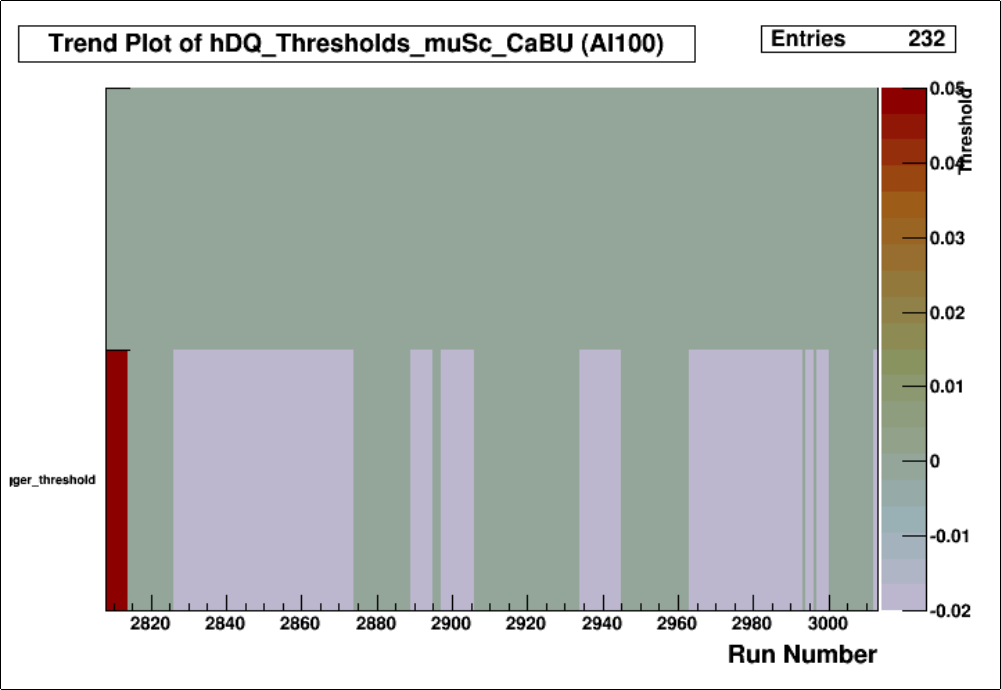
\includegraphics[width=\linewidth]{figs/al100/cabu_thresh}
    \caption{}\label{fig:al100_cabu_thresh}
  \end{subfigure}%
  \begin{subfigure}{0.4\textwidth}
    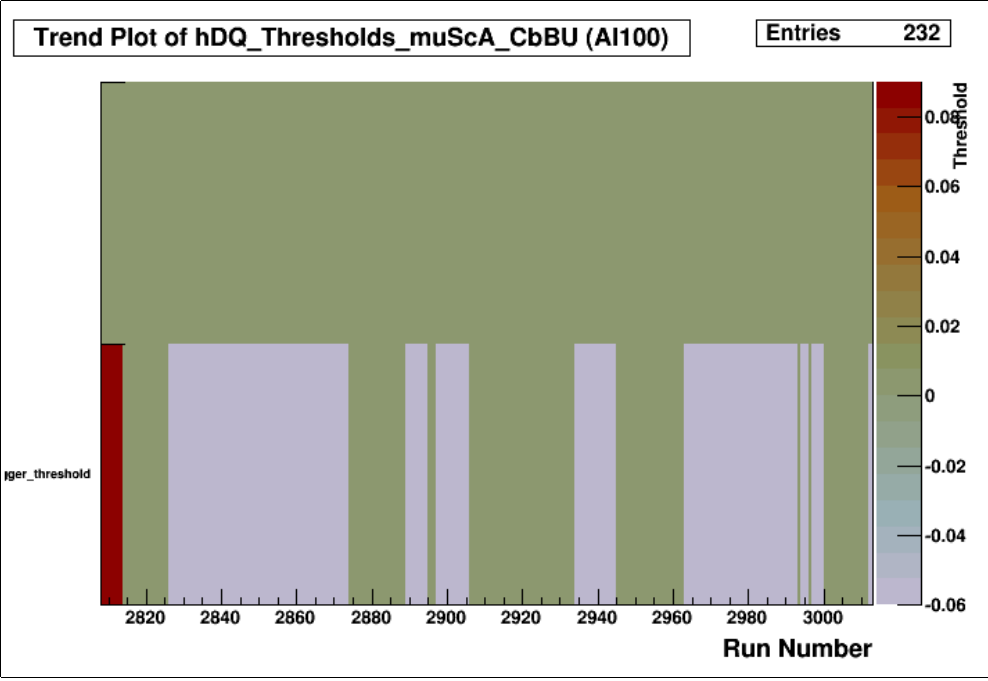
\includegraphics[width=\linewidth]{figs/al100/cbbu_thresh}
    \caption{}\label{fig:al100_cbbu_thresh}
  \end{subfigure}
  \begin{subfigure}{0.4\textwidth}
    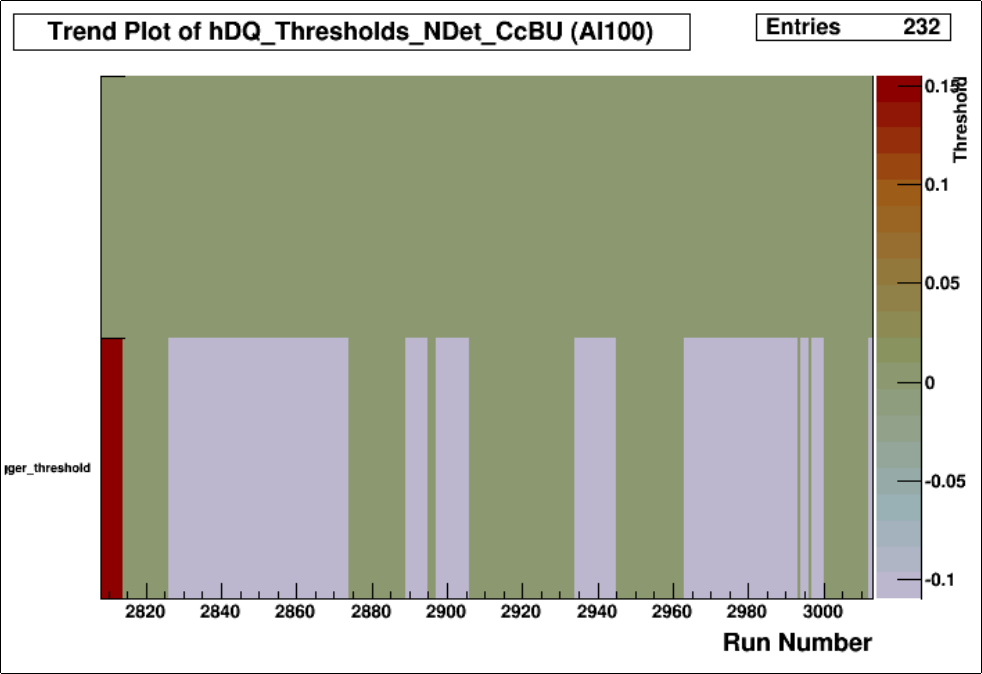
\includegraphics[width=\linewidth]{figs/al100/ccbu_thresh}
    \caption{}\label{fig:al100_ccbu_thresh}
  \end{subfigure}%
  \begin{subfigure}{0.4\textwidth}
    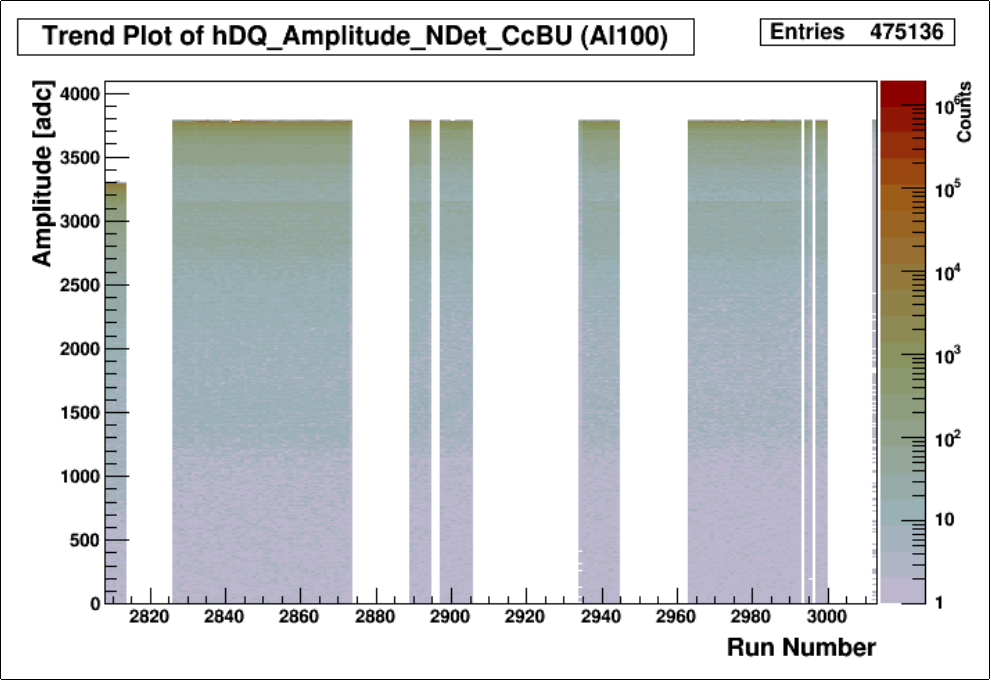
\includegraphics[width=\linewidth]{figs/al100/ndet_amp}
    \caption{}\label{fig:al100_ndet_amps}
  \end{subfigure}
  \caption{BU CAEN thresholds changed near the first runs of the Al100 dataset \ref{fig:al100_cabu_thresh}-\ref{fig:al100_ccbu_thresh}
    and the amplitude change that resulted from the NDet pedestal change \ref{fig:al100_ndet_amps}.}
  \label{fig:al100_caen_changes}
\end{figure}


\subsubsection{FADC Threshold Changes}
\label{sec:al100_threshold_changes}

The thresholds were changed between runs 2873 and 2889 (elog:555, \ref{fig:al100_thresholds_change}),
which greatly changed the rates in some of the silicon detectors \ref{fig:al100_rates}.
Many detectors had no hits before the thresholds were lowered. This caused an understandable
change in the amplitude spectra of certain channels as well, an example of which can
be seen in \ref{fig:al100_sir11s_amps}.

\begin{figure}
  \centering
  \begin{subfigure}{0.5\textwidth}
    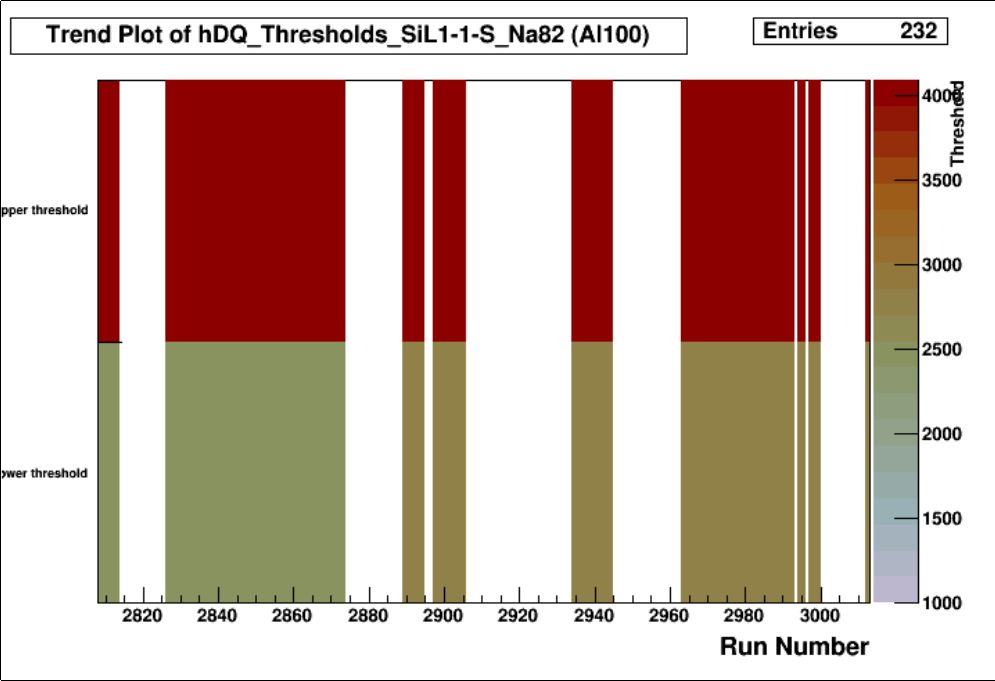
\includegraphics[width=0.8\linewidth]{figs/al100/sil11s_thresh}
    \caption{}\label{fig:al100_sil11s_thresh}
  \end{subfigure}%
  \begin{subfigure}{0.5\textwidth}
    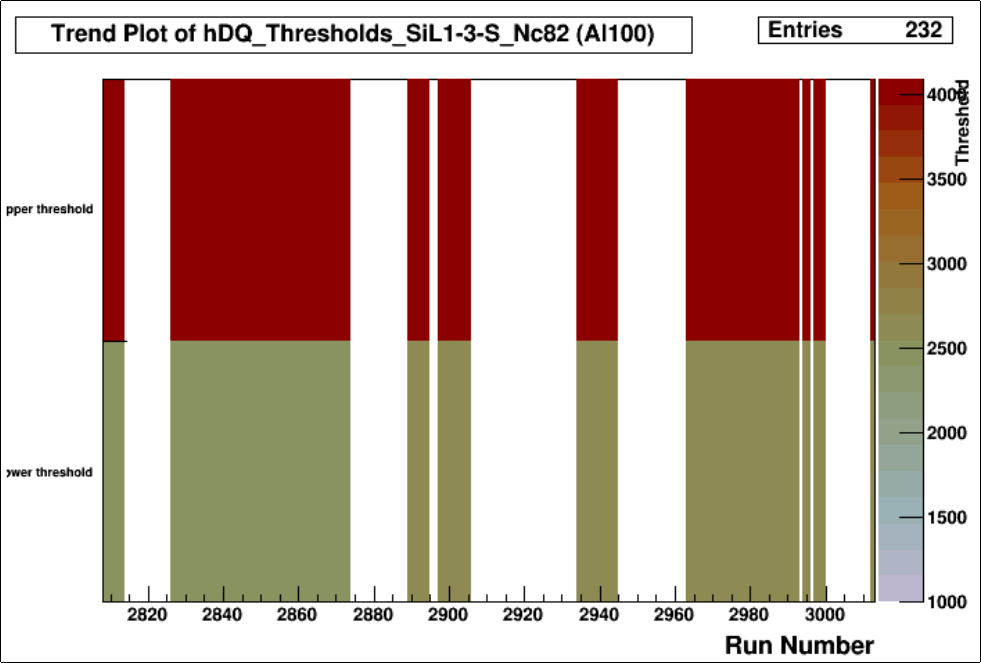
\includegraphics[width=0.8\linewidth]{figs/al100/sil13s_thresh}
    \caption{}\label{fig:al100_sil13s_thresh}
  \end{subfigure}
  \begin{subfigure}{0.5\textwidth}
    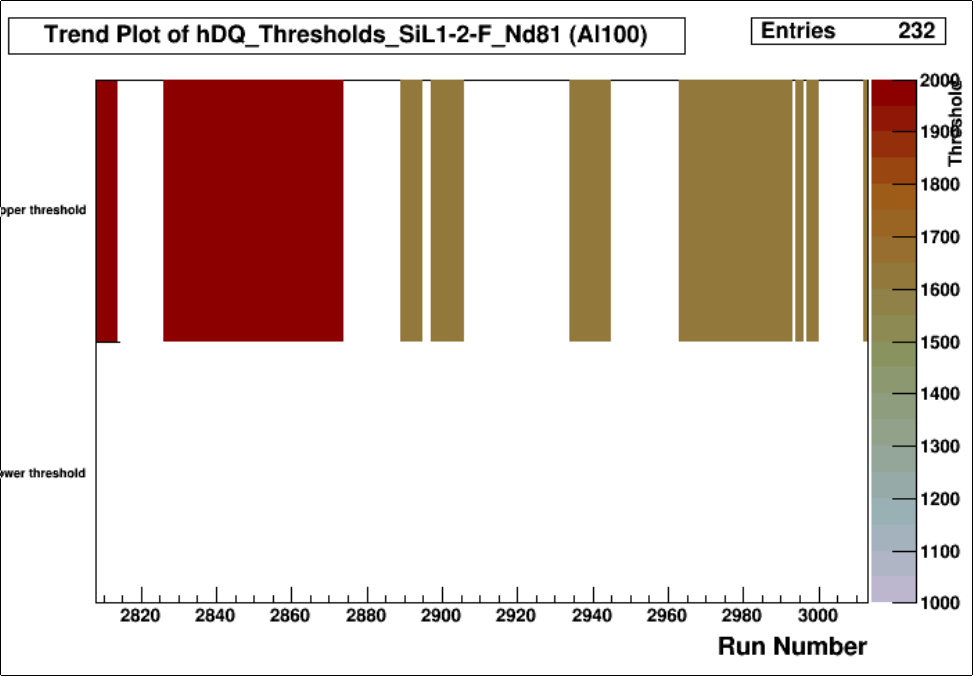
\includegraphics[width=0.8\linewidth]{figs/al100/sil12f_thresh}
    \caption{}\label{fig:al100_sil12f_thresh}
  \end{subfigure}%
  \begin{subfigure}{0.5\textwidth}
    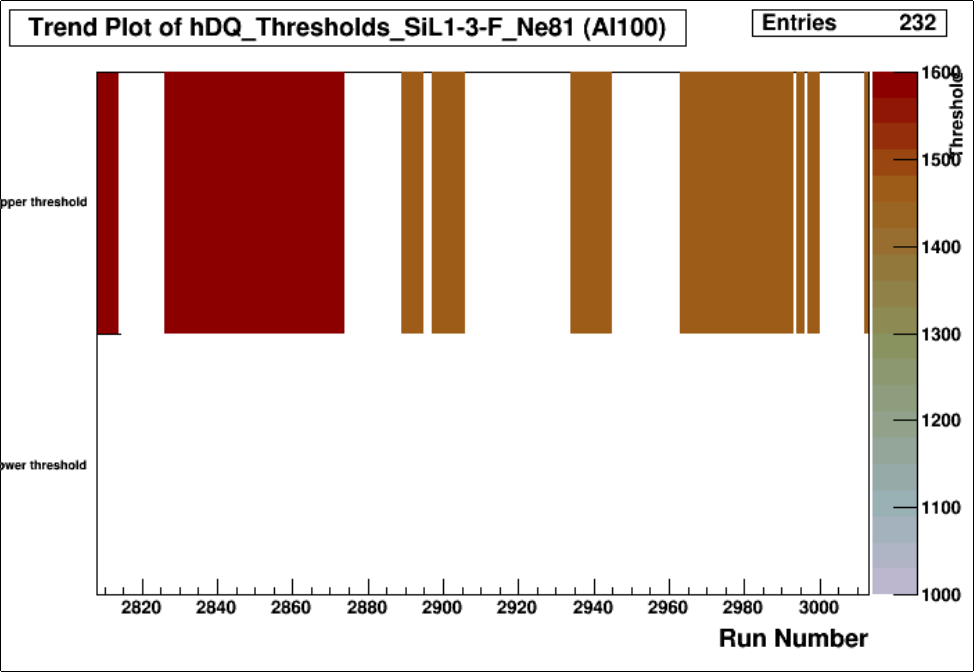
\includegraphics[width=0.8\linewidth]{figs/al100/sil13f_thresh}
    \caption{}\label{fig:al100_sil13f_thresh}
  \end{subfigure}
  \begin{subfigure}{0.5\textwidth}
    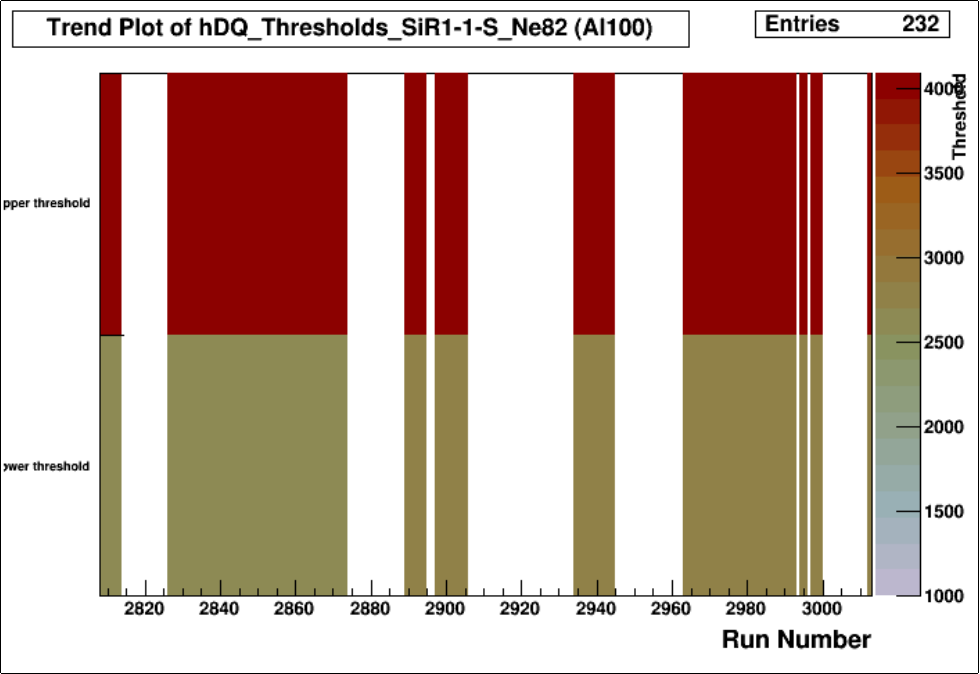
\includegraphics[width=0.8\linewidth]{figs/al100/sir11s_thresh}
    \caption{}\label{fig:al100_sir11s_thresh}
  \end{subfigure}
  \caption{Examples of thresholds in silicon channels that were changed between runs to
    get better agreement between number of events the slow and fast channels for a given
    silicon detector saw.}
  \label{fig:al100_thresholds_change}
\end{figure}

\begin{figure}
  \centering
  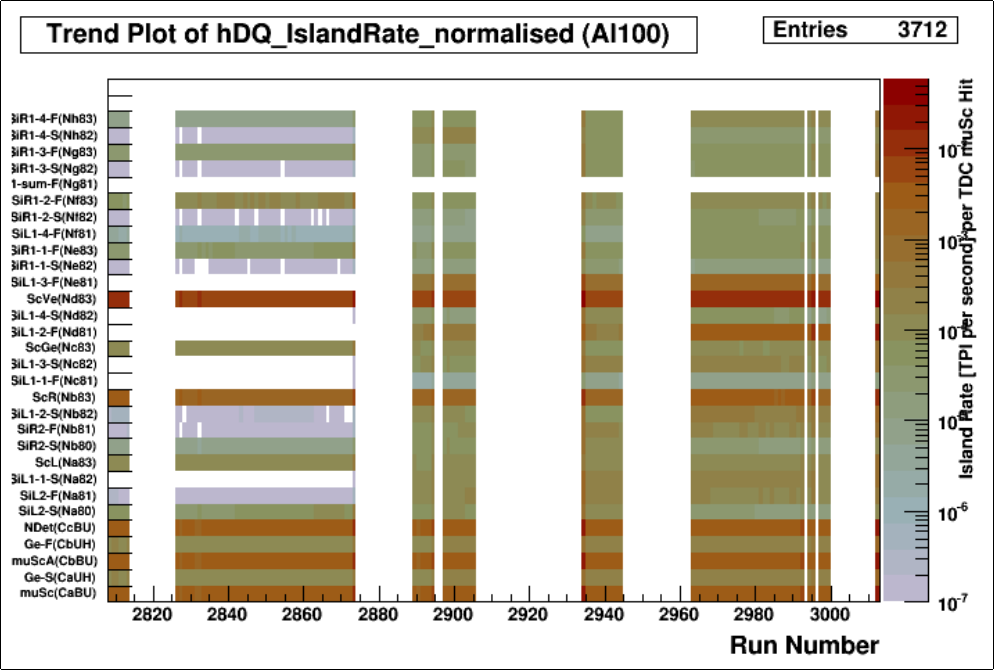
\includegraphics[width=0.9\linewidth]{figs/al100/rates}
  \caption{Rates in all detectors for Al100 dataset.}
  \label{fig:al100_rates}
\end{figure}

\begin{figure}
  \centering
  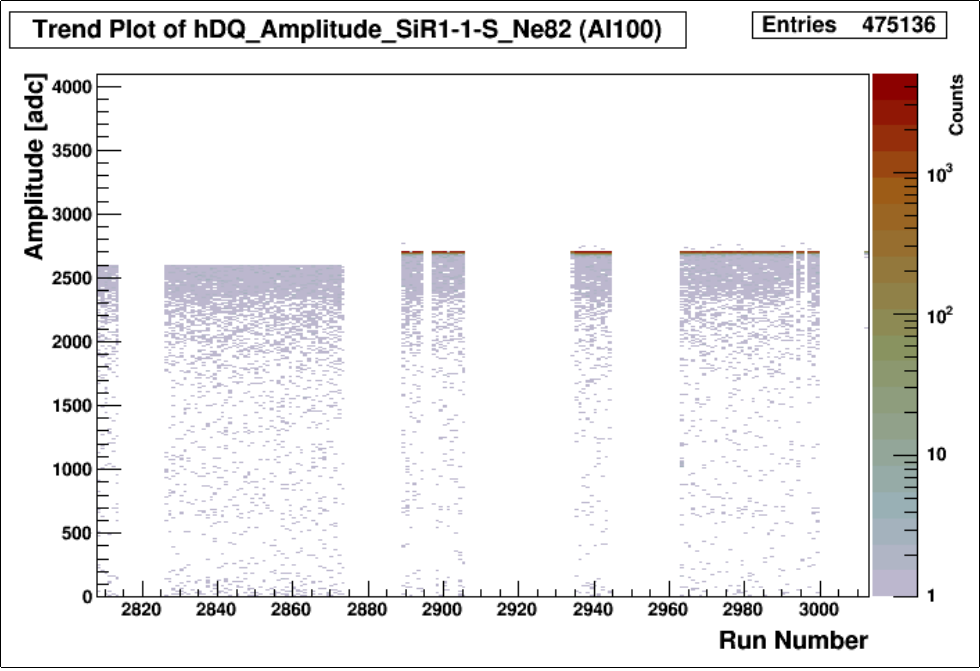
\includegraphics[width=0.9\linewidth]{figs/al100/sir11s_amps}
  \caption{An example of how the amplitudes changes after the thresholds
    were adjusted after run 2873.}
  \label{fig:al100_sir11s_amps}
\end{figure}

\subsubsection{Buffer Overflow}
\label{sec:al100_buffer_overflow}
\paragraph{FADC 0x83}
FADC 0x83 saw 100\% overflow for the entirety of this dataset \ref{fig:al100_buffer_overflow}.
The attached detectors were ScVe, ScR, ScL, ScGe, SiR1-1-F, SiR1-2-F, SiR1-3-F, and SiR1-4-F.
The most agregious offender was ScVe and can be seen in \ref{fig:al100_rates}. A sympton of this
is that we had many data from the beginning of any given event as illustrated in
\ref{fig:al100_scve_timestamps}.

\begin{figure}
  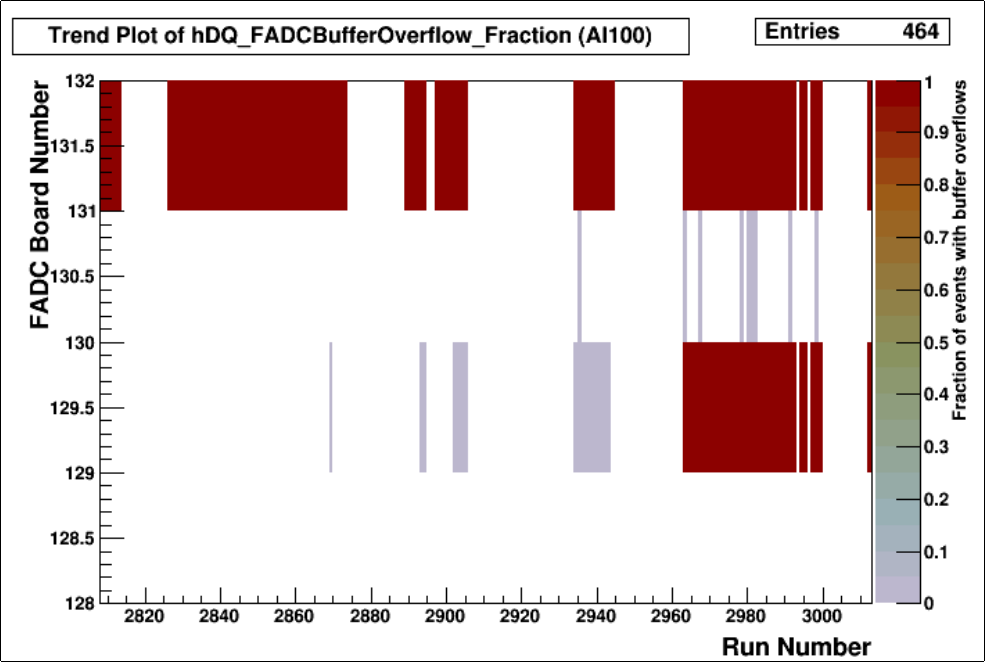
\includegraphics[width=0.9\linewidth]{figs/al100/buffer_overflow}
  \caption{FADC 0x83 had 100\% buffer overflow
    for the entirety of the dataset. FADC 0x81 had 100\% buffer overflow when
    issues with certain detectors started popping up.}
  \label{fig:al100_buffer_overflow}
\end{figure}

\begin{figure}
  \begin{subfigure}{0.5\textwidth}
    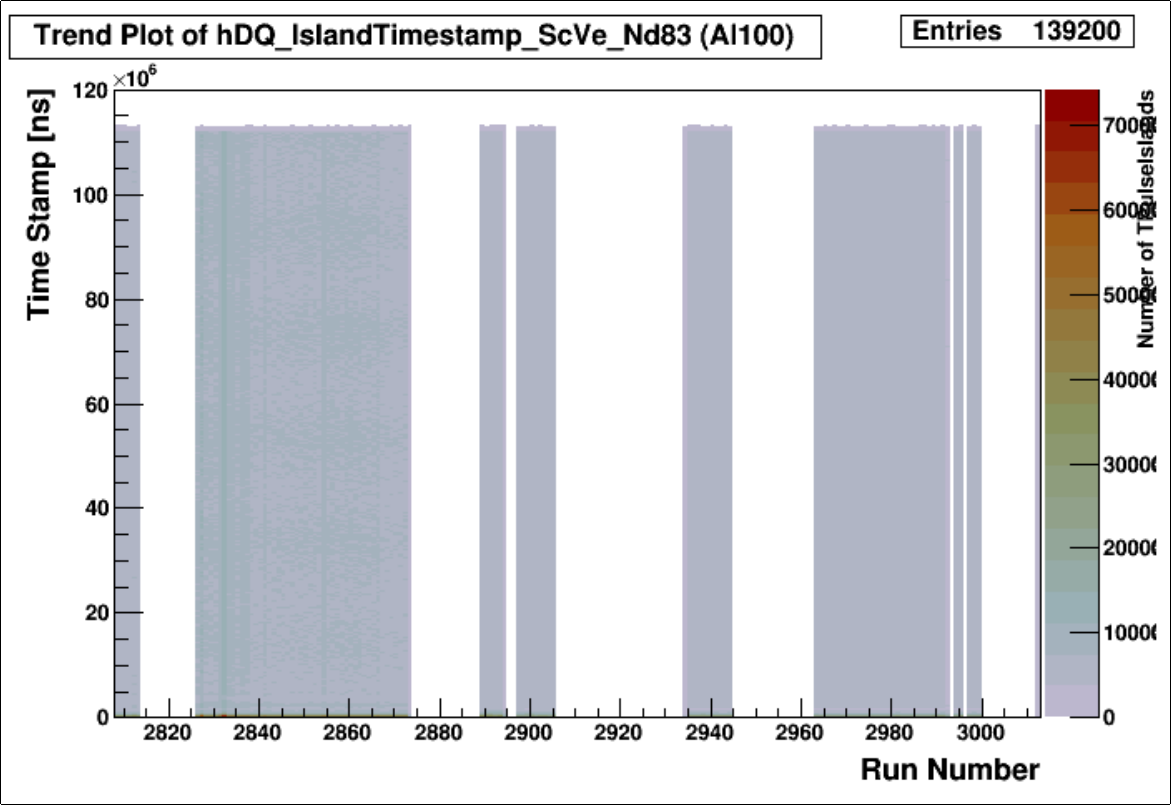
\includegraphics[width=0.9\linewidth]{figs/al100/scve_timestamps}
  \end{subfigure}%
  \begin{subfigure}{0.5\textwidth}
    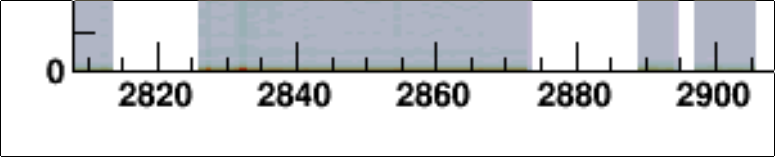
\includegraphics[width=0.9\linewidth]{figs/al100/scve_timestamps_zoom}
  \end{subfigure}
  \caption{On the left we see the timestamp distribution for the ScVe detector,
    and if we zoom in on the right we see the MIDAS events were very front-loaded
    as the data buffer on FADC 0x83 filled up at the beginning of an event.
    One has to squint to be sure, but it is dark red near the horizontal axis.}
  \label{fig:al100_scve_timestamps}
\end{figure}

\paragraph{FADC 0x81}
For the overflow that started later on FADC 0x81, the problem seems to be with the SiL1-2-F
detector. Both the fast and slow channels seemed to be acting up, though only the fast channel
led to buffer overflows. Evidence that both channels were causing problems can be seen
in \ref{fig:al100_sil12_n}.

The reason for this is unknown, and it is being investigated.


\begin{figure}
  \begin{subfigure}{0.5\textwidth}
    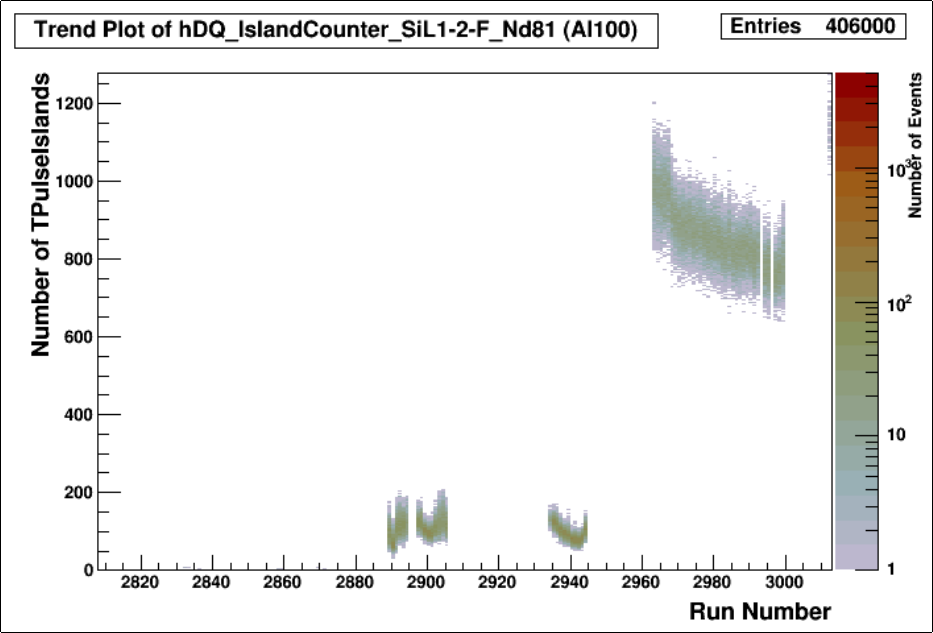
\includegraphics[width=0.9\linewidth]{figs/al100/sil12f_n}
  \end{subfigure}%
  \begin{subfigure}{0.5\textwidth}
    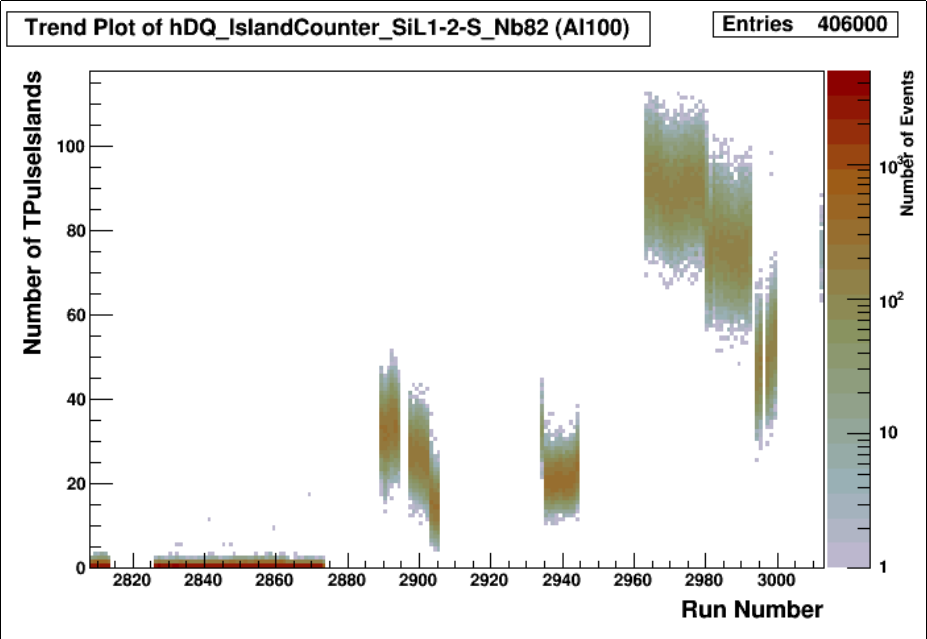
\includegraphics[width=0.9\linewidth]{figs/al100/sil12s_n}
  \end{subfigure}
  \caption{Number of TPIs from SiL1-2 both fast and slow channels. There
    was a drastic increase afer run 2963.}
  \label{fig:al100_sil12_n}
\end{figure}


\subsubsection{Packet Loss}
\label{sec:al100_packet_loss}

The only appreciable packet loss was on FADC 0x82 as evident in \ref{fig:al100_packet_loss}.
In practice we've tended to not concern outselve too much if this is below 10\%, which
happens after the thresholds have been adjusted.

\begin{figure}
  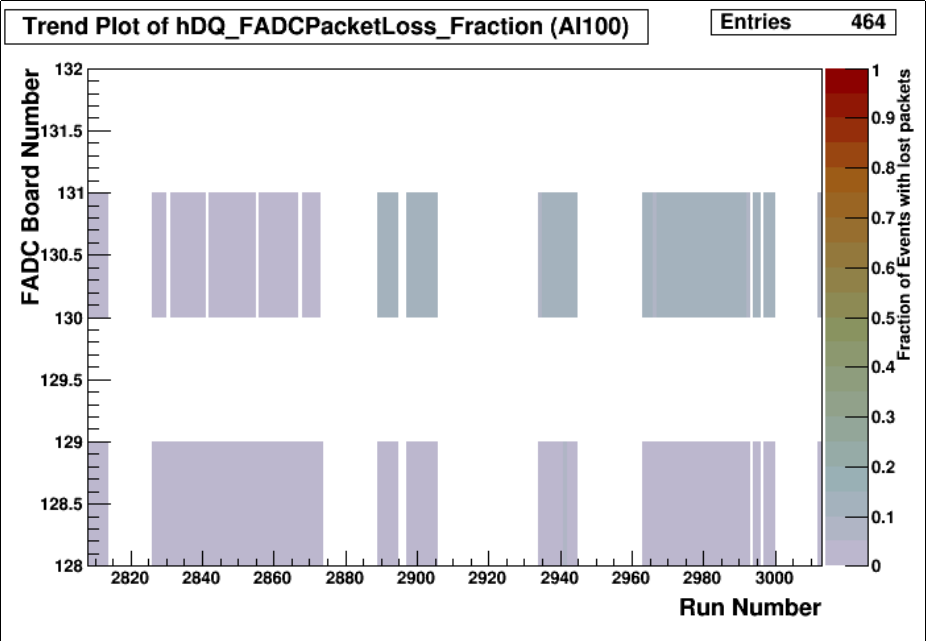
\includegraphics[width=0.9\linewidth]{figs/al100/packet_loss}
  \caption{Packet loss becomes noticeably higher after the thresholds get adjusted for
    FADC 0x82.}
  \label{fig:al100_packet_loss}
\end{figure}


\subsubsection{Unstable muSc}

The muSc rate according to the CAEN TDC data seems to fluctuate after the thresholds
on the FADCs have been adjusted. Considering the TDC is not related to the FADCs,
this could mean that during the downtime something happened to the beam (it did go down
several times during the remainder of the data set). This can be seen in figure \ref{fig:al100_musc_rate}.

\begin{figure}
  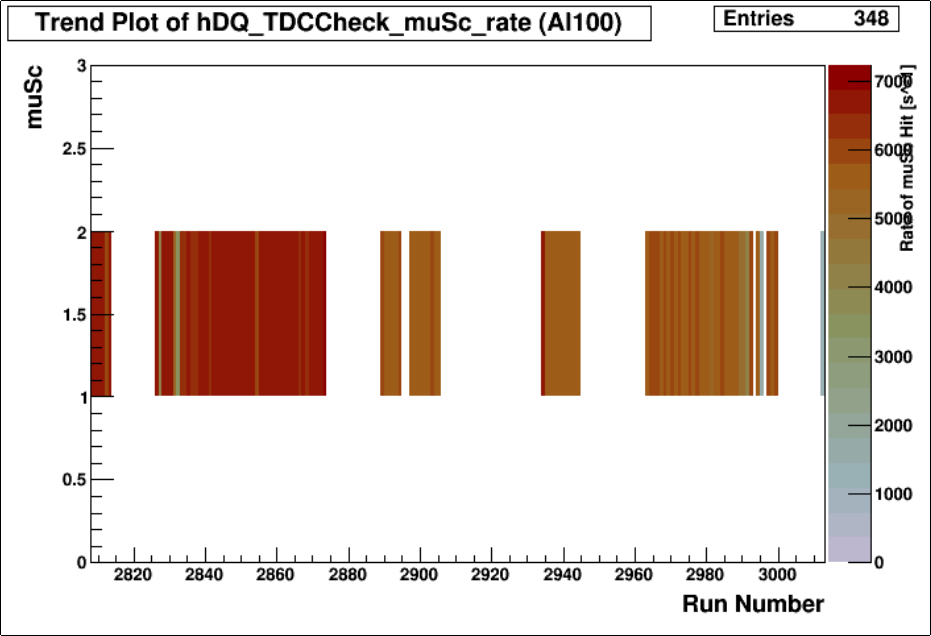
\includegraphics[width=0.9\linewidth]{figs/al100/musc_rate}
  \caption{In the latter half of this data set, one might
    observe the rate in the muSc to be less consistent. Though
    the exact magnitude of the fluctuations is difficult
    to tell from this plot.}
  \label{fig:al100_musc_rate}
\end{figure}



\subsubsection{Noisy Germanium}
\label{sec:al100_ge_noisy}

After run 2894 the germanium detector got much noisier. The reason for this is unknown.
Between runs 2894 and 2897 two ambient runs were taken and the germanium was refilled with liquid nitrogen.
The noise manifested itself both in number of pulse islands and length of pulse islands, as can be
seen in \ref{fig:al100_ge_noise}. 

\begin{figure}
  \begin{subfigure}{0.5\textwidth}
    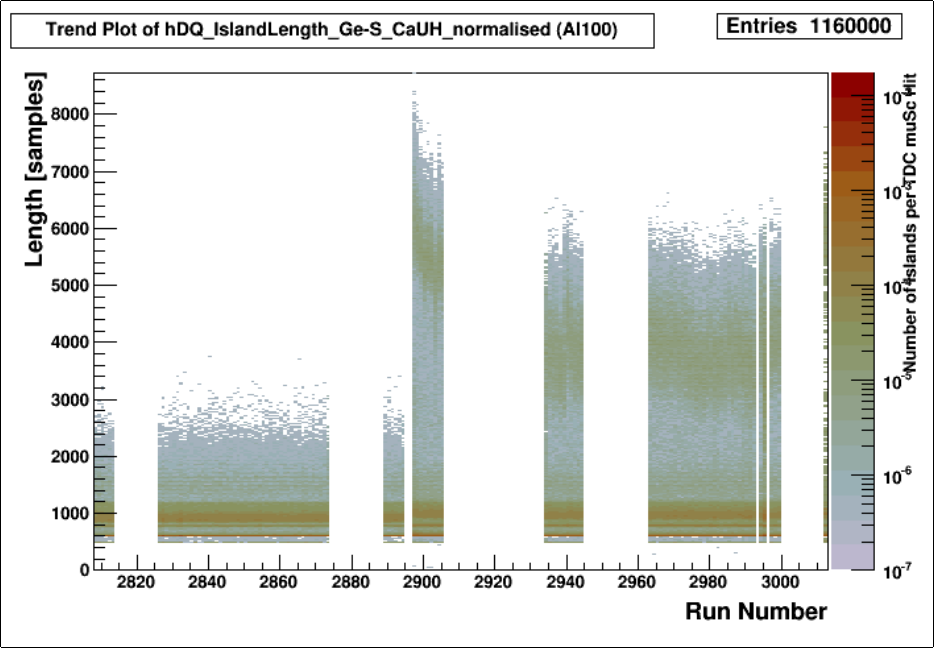
\includegraphics[width=0.9\linewidth]{figs/al100/ges_length}
  \end{subfigure}%
  \begin{subfigure}{0.5\textwidth}
    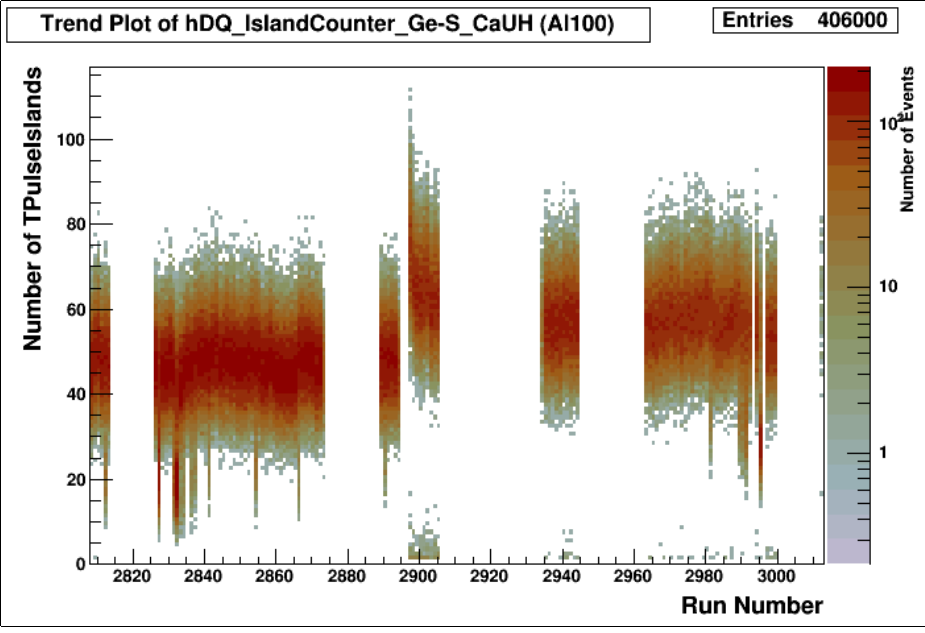
\includegraphics[width=0.9\linewidth]{figs/al100/ges_n}
  \end{subfigure}
  \caption{The noise in the germanium for the later half
    of the dataset can be seen here. On the left we see a drastic
    increase in the TPI length, and a mild increase in the number
    of TPIs.}
  \label{fig:al100_ge_noise}
\end{figure}


\subsubsection{Strange Silicon Amplitudes}
\label{sec:al100_silicon_amps}

The amplitudes for some of the silicon channels (most notably SiL1-2-F) seemed to dip inexplicably
for some runs \ref{fig:al100_sil12f_amps}.
This could perhaps be related to issue \ref{sec:al100_buffer_overflow}. Other channels
had interesting behavior like this, but less frequently. Additionally, the pedestals
for this channel were different than for other channels on the same board.

\begin{figure}
  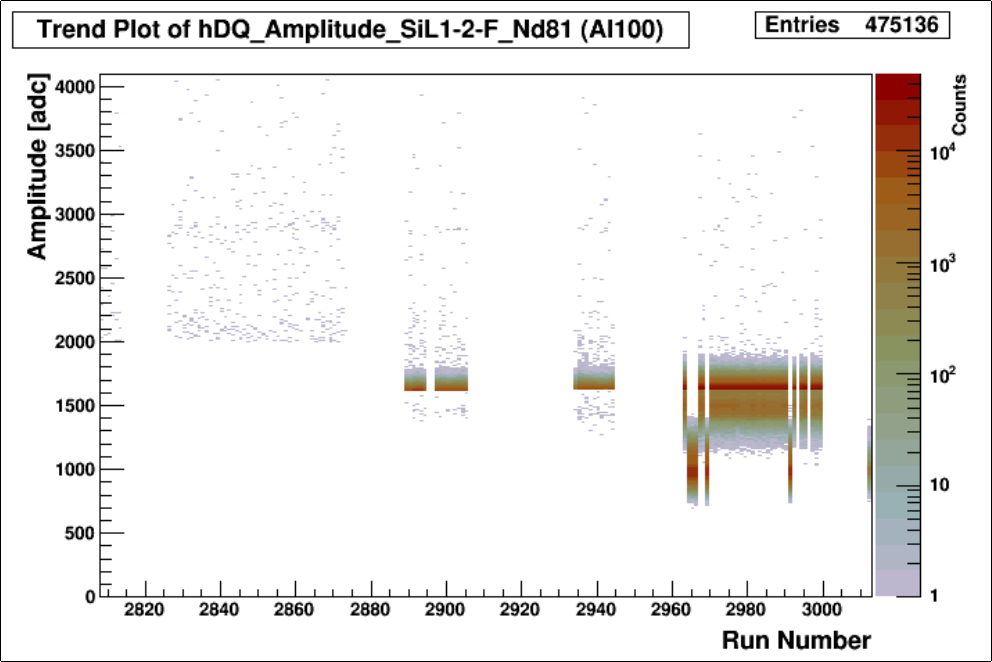
\includegraphics[width=0.9\linewidth]{figs/al100/sil12f_amp}
  \caption{There is something funny going on with the amplitudes of this channel.
    The pedestal for this channel is also different than the other 0x81 channels.}
  \label{fig:al100_sil12f_amps}
\end{figure}


\subsubsection{Timestamp Oscillations}
\label{sec:al100_timestamp_oscillations}

There seem to be bands in the timestamps plot \ref{fig:al100_timestamp_banding}.
There is 50 Hz noise in the Ge-S channel, but the more frequent bands
we have not been able to identify the source of.

\begin{figure}
  \centering
  \begin{subfigure}{0.5\textwidth}
    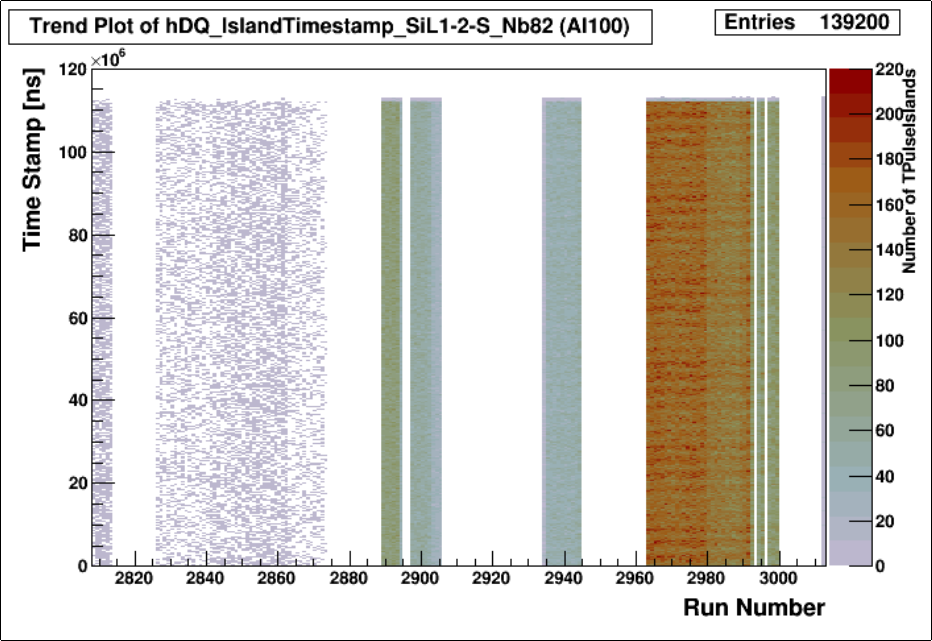
\includegraphics[width=0.9\linewidth]{figs/al100/sil12s_timestamps}
  \end{subfigure}%
  \begin{subfigure}{0.5\textwidth}
    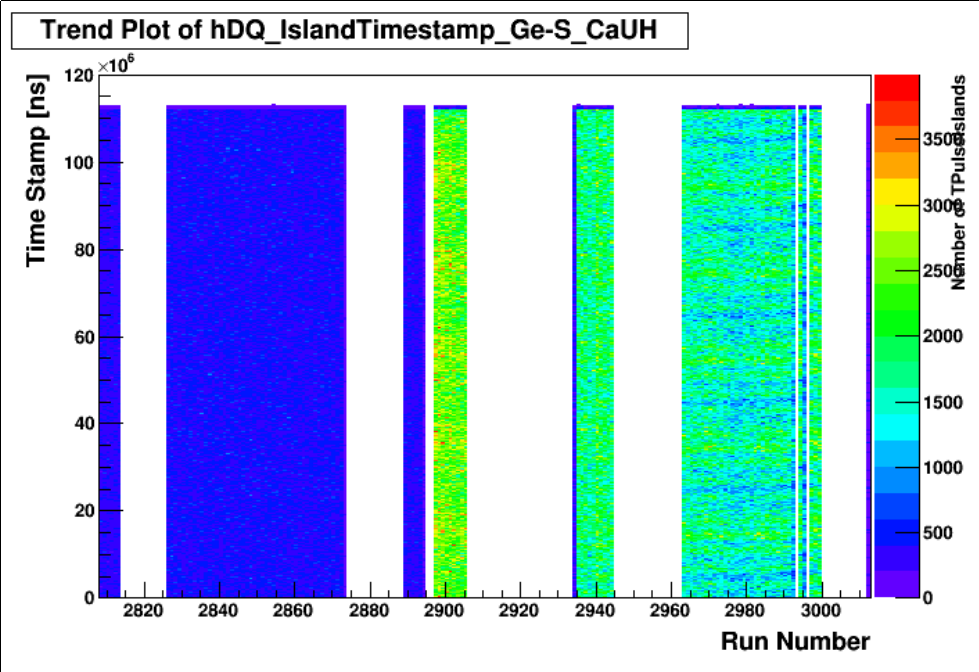
\includegraphics[width=0.9\linewidth]{figs/al100/ges_timestamps}
  \end{subfigure}
  \caption{On the left we can see some bands in the time distribution
    of SiL-1-2-S hits with respect to the start of a MIDAS event. It's
    not immediately clear what the culprit is. On the right we see the
    same for the Ge-S channel, with some obvious 50 Hz noise mixed in
    with the sanem noise from the silicon on the left.}
  \label{fig:al100_timestamp_banding}
\end{figure}


\subsubsection{Run 3012}

The problems with run 3012, the last run in this data set, were numerous. Many of these may stem
from the livetime for the run being so short (47 seconds according to the run database, zero according
to our livetime histogram). The noise was bad.


\subsection{Conclusions}

Thresholds were adjusted several times during this data set, most noticeably during the beginning.
It has been suggested we split the dataset at 2880. If both parts of the dataset give us the same physics results, 

The final run (3012) can be excluded if we want.

%%%%%%%%%%%%%%%%%%%%%%%%%%%%%%%%%%%%%%%%%%%%%%%%%%%%%%%%%%%%%%%

\section{Al50 - A (with NDet)}
\begin{itemize}
  \item Aluminum
  \item 50 $\mu$m thick
  \item 10 cm $\times$ 10 cm
  \item Momentum scale factor 1.07
  \item Runs: 3442-3456
\end{itemize}

\subsection{Issues}
\subsubsection{Consistently Low Rates}
\label{sec:al50andet2_rates}

This run came right after some $\mu^+$ runs. Whether the magnets were't tuned properly, or the slits were close, or thresholds were far too
high, the rates were awfully low as seen in \ref{fig:al50andet2_rates}. The rates were also a bit higher near the beginning, and
this has not been explained yet either.

\begin{figure}
  \centering
  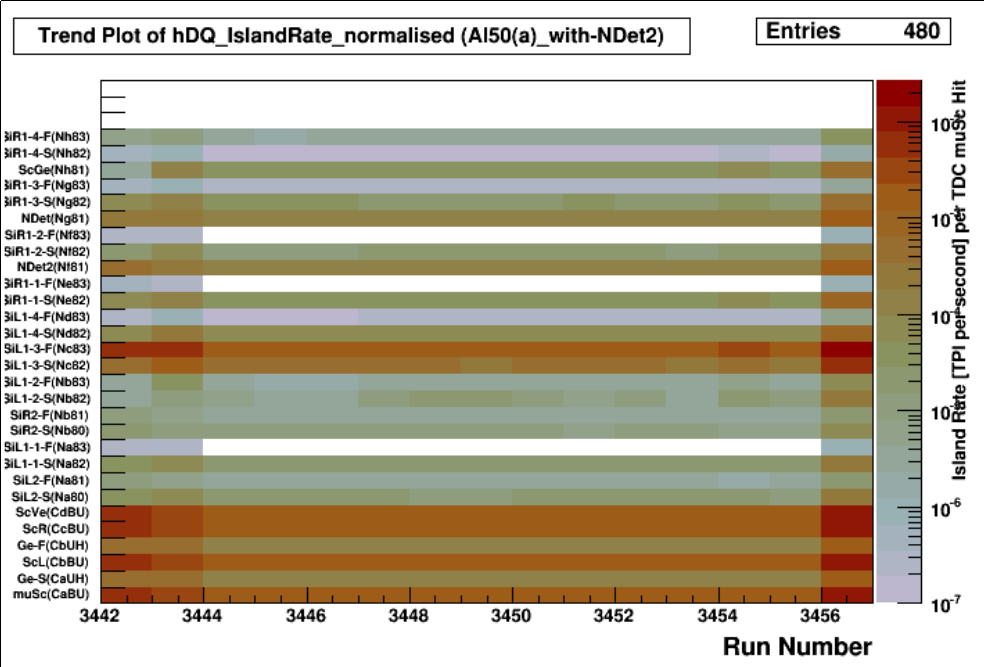
\includegraphics[width=0.9\linewidth]{figs/al50andet2/rates}
  \caption{Rates are low (~0) for some detectors.}
  \label{fig:al50andet2_rates}
\end{figure}


\subsubsection{Odd Amplitudes for first two runs}
\label{sec:al50andet2_amps}

The first run has a lower cutoff in the amplitudes for some of the detectors, and the second run also has some stuff going on. This
can be seen in \ref{fig:al50andet2_amps}.

\begin{figure}
  \centering
  \begin{subfigure}{0.5\textwidth}
    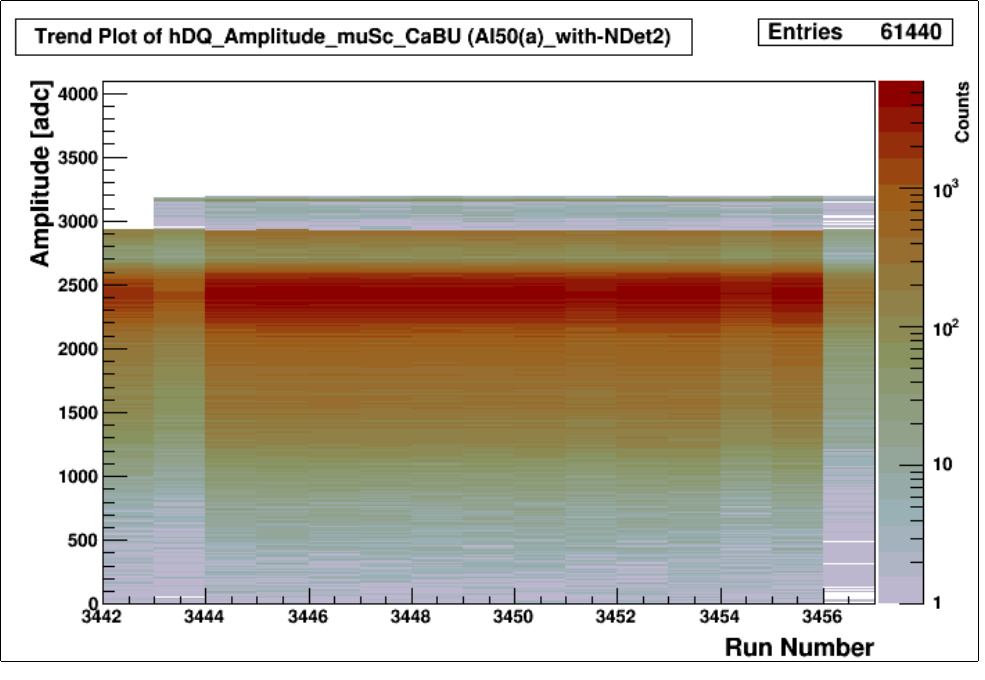
\includegraphics[width=0.9\linewidth]{figs/al50andet2/musc_amp}
  \end{subfigure}%
  \begin{subfigure}{0.5\textwidth}
    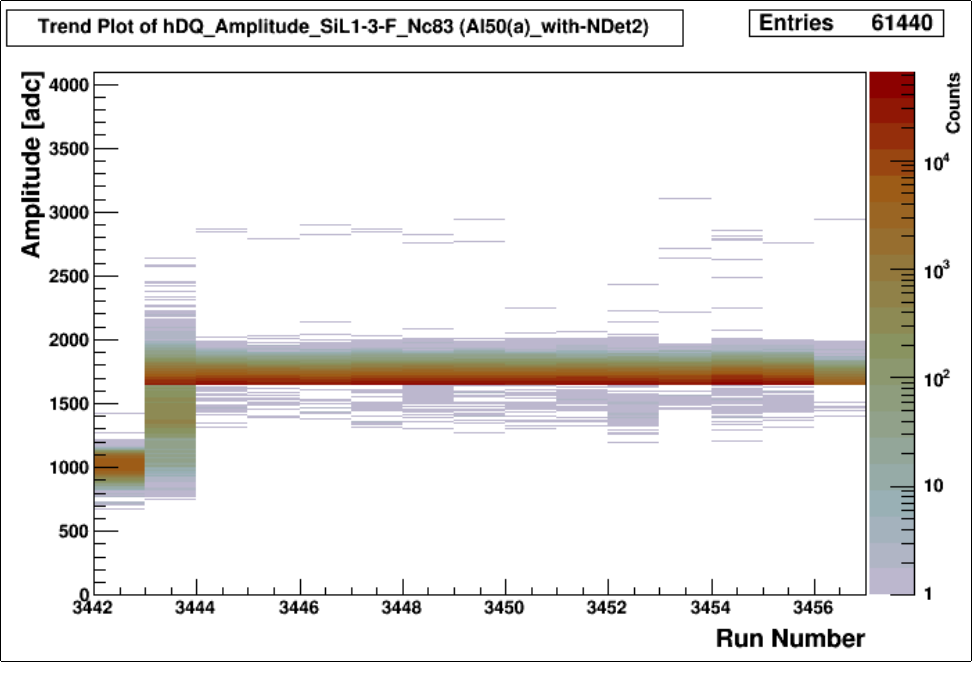
\includegraphics[width=0.9\linewidth]{figs/al50andet2/sil13f_amp}
  \end{subfigure}
  \begin{subfigure}{0.5\textwidth}
    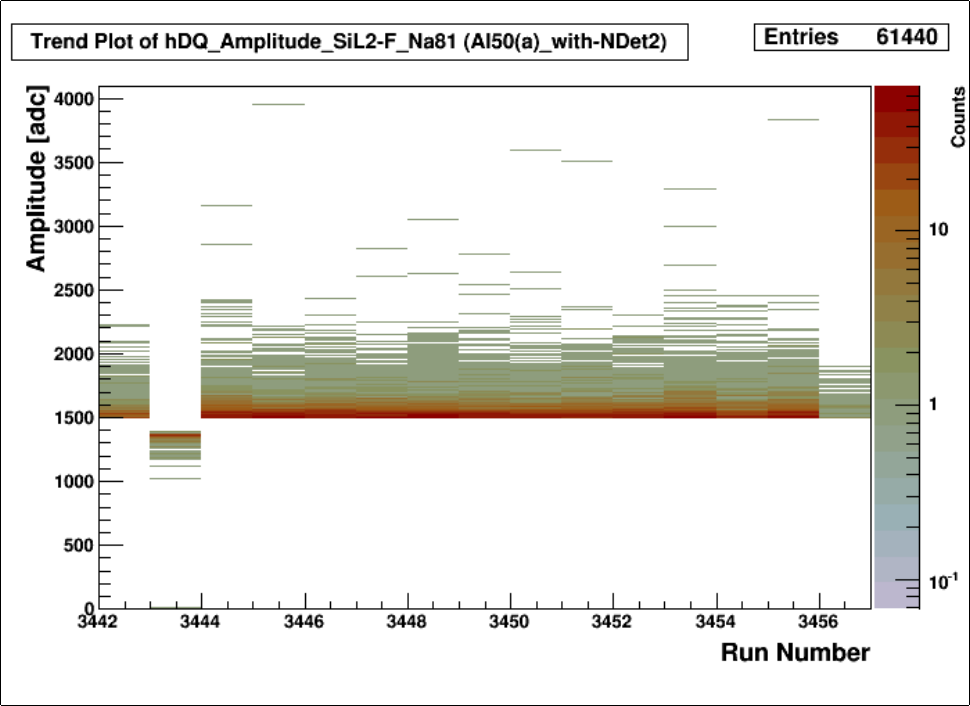
\includegraphics[width=0.9\linewidth]{figs/al50andet2/sil2f_amp}
  \end{subfigure}%
  \begin{subfigure}{0.5\textwidth}
    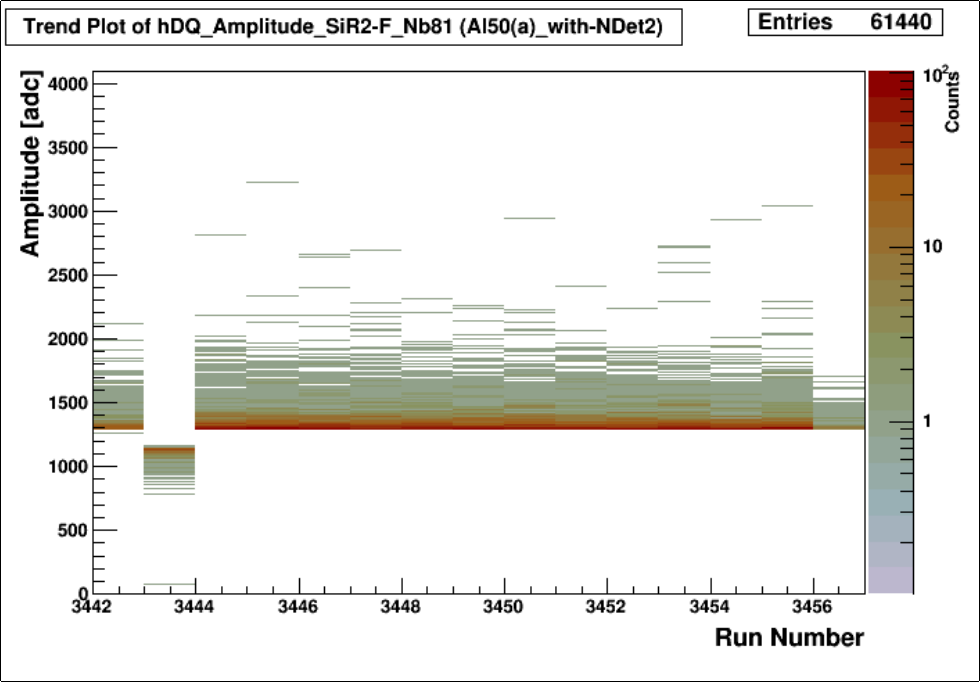
\includegraphics[width=0.9\linewidth]{figs/al50andet2/sir2f_amp}
  \end{subfigure}
  \caption{The first two runs show interesting amplitude cutoffs for some detectors.}
  \label{fig:al50andet2_amps}
\end{figure}


\subsubsection{Short pulse islands}
\label{sec:al50andet2_length}

Some detectors seemed to have very short pulse islands, the worst offender being SiL1-3-F as seen in \ref{fig:al50andet2_length}.
This should be examined.

\begin{figure}
  \centering
  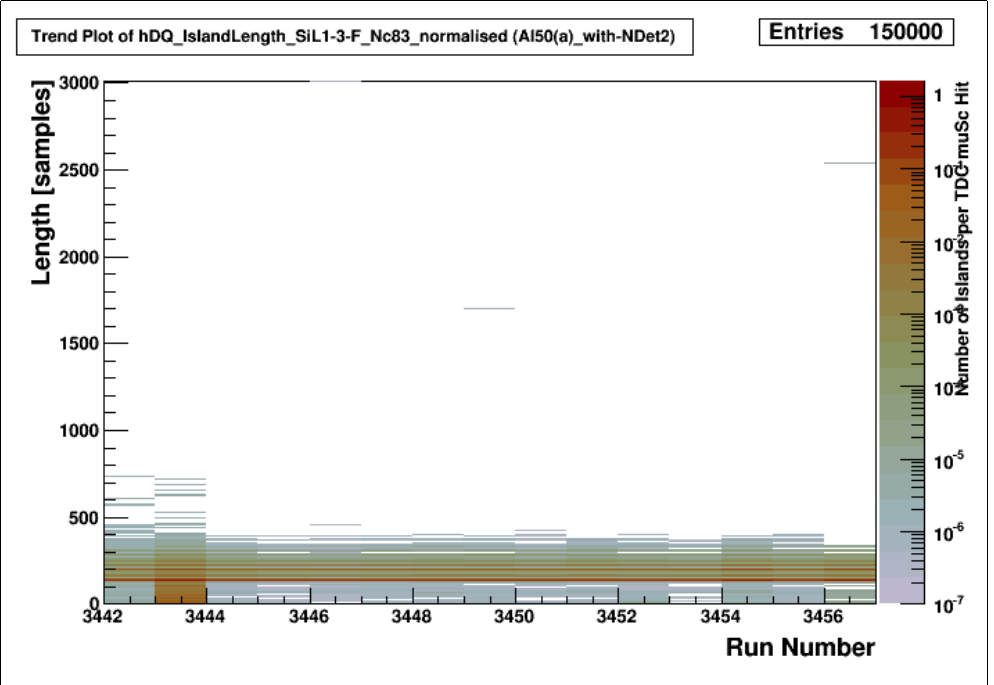
\includegraphics[width=0.9\linewidth]{figs/al50andet2/sil13f_length}
  \caption{The island lengths seem to go close to zero, and this should not be possible}
  \label{fig:al50andet2_length}
\end{figure}

\subsection{Conclusion}

This run wasn't that long, and had a few issues. It occured just after a $\mu^+$ run and so the rate was
much lower than it had been before for many detectors. Instead of analysing this piecemeal, we can continue to process
it but keep it low priority; make it a so-called ``silver'' dataset entirely.

%%%%%%%%%%%%%%%%%%%%%%%%%%%%%%%%%%%%%%%%%%%%%%%%%%%%%%%%%%%%%%%

\section{Al50 - A (Without NDet)}
\begin{itemize}
  \item Aluminum
  \item 50 $\mu$m thick
  \item 10 cm $\times$ 10 cm
  \item Momentum scale factor 1.07
  \item Runs:
    3101-3104, 3110-3117, 3141-3144,
    3146-3149, 3153-3156, 3160-3167,
    3183-3226, 3238-3257, 3263-3295,
    3322-3324, 3326-3329
\end{itemize}


\subsection{Issues}

\subsubsection{Pulse Island Lengths Inconsistent}
\label{sec:al50a_tpi_length_incosnsistent}
For a number of runs, the pulse island lengths got a bit erratic as in \ref{fig:al50a_erratic_lengths}.
A red flag is that the pulse island lengths are, for some runs, consistently below the minimum length we would expect.
Some other detectors, as seen in \ref{fig:al50a_consistent_bad_lengths}, have lengths below the expected but
are consistent throughout the entire dataset, giving it a feeling of normalcy. However we do not yet know why this happens.

\begin{figure}
  \centering
  \begin{subfigure}{0.5\textwidth}
    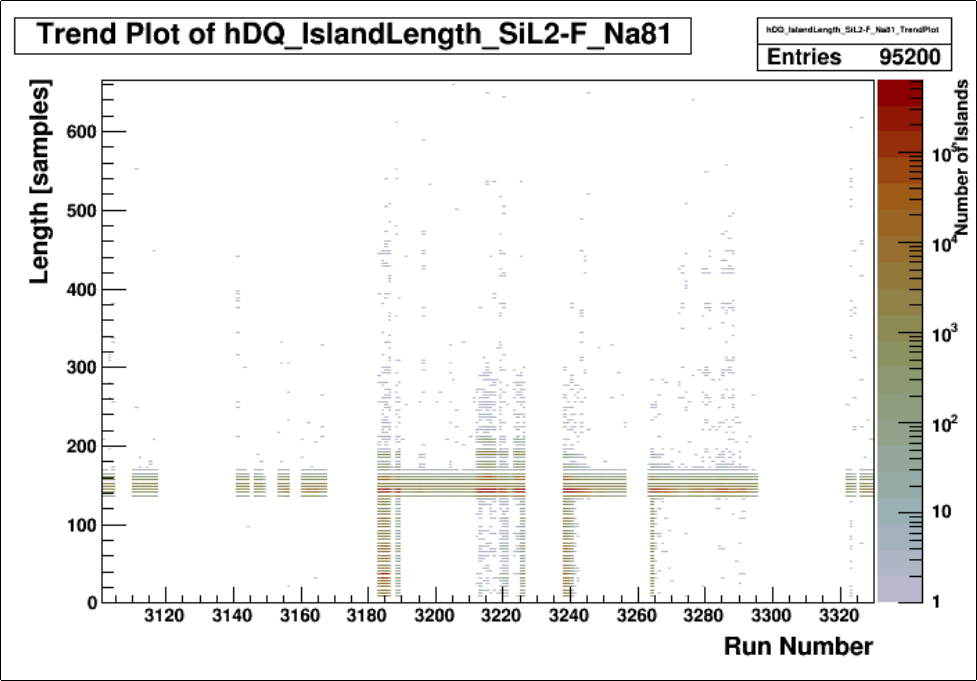
\includegraphics[width=0.9\linewidth]{figs/al50a/sil2f_length}
  \end{subfigure}%
  \begin{subfigure}{0.5\textwidth}
    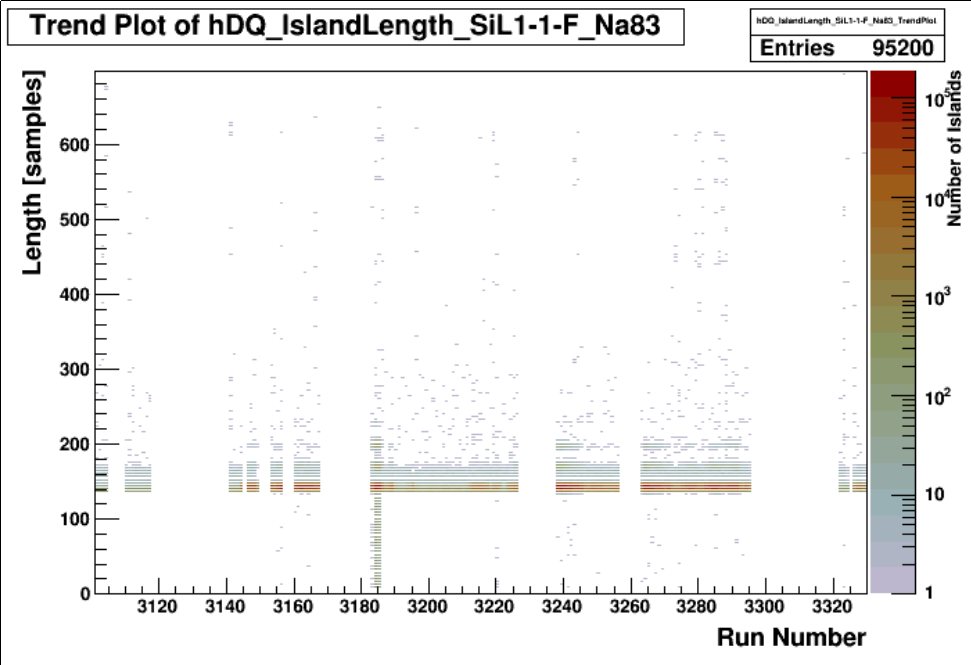
\includegraphics[width=0.9\linewidth]{figs/al50a/sil11f_length}
  \end{subfigure}

  \begin{subfigure}{0.5\textwidth}
    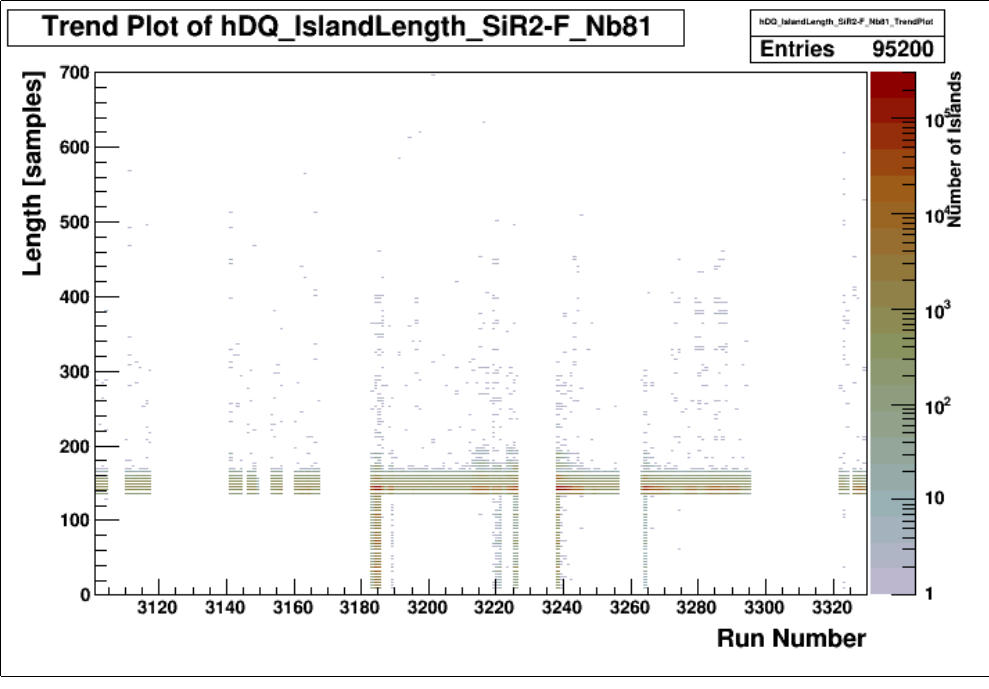
\includegraphics[width=0.9\linewidth]{figs/al50a/sir2f_length}
  \end{subfigure}%
  \begin{subfigure}{0.5\textwidth}
    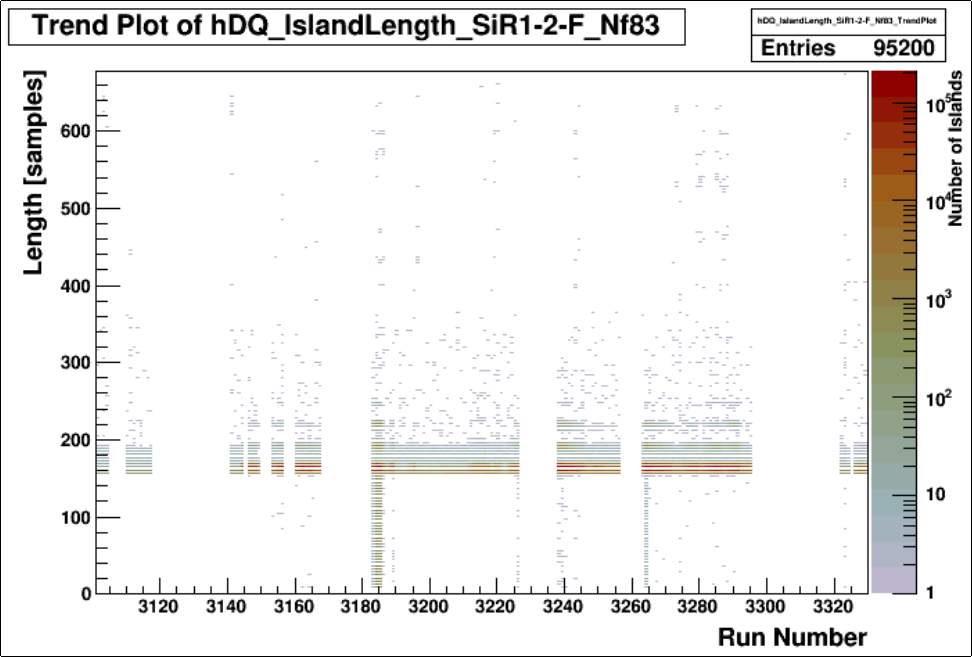
\includegraphics[width=0.9\linewidth]{figs/al50a/sir12f_length}
  \end{subfigure}
  \caption{An example of how, for some of the runs, the pulse island lengths could vary quite a bit.}
  \label{fig:al50a_erratic_lengths}
\end{figure}

\begin{figure}
  \centering
  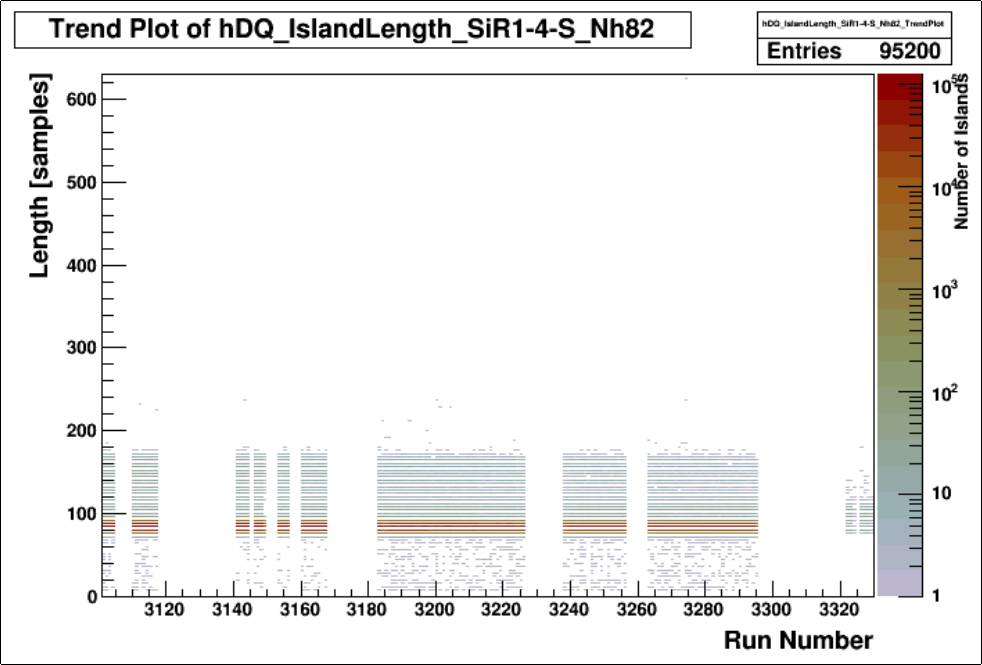
\includegraphics[width=0.9\linewidth]{figs/al50a/sir14s_length}
  \caption{Instead of being erratic, some pulse island lengths are consistently less than what we'd expect.}
  \label{fig:al50a_consistent_bad_lengths}
\end{figure}

\subsubsection{Pulse Island Length Banding}
\label{sec:al50a_tpi_length_bands}
One can additionally see that the pulse island lengths in \ref{fig:al50a_erratic_lengths} and \ref{fig:al50a_consistent_bad_lengths}
bunch up. This could be because the atom in the FADC settings are ``stretch samples'' which are, in fact, two samples.
But this has not been confirmed.

\subsubsection{Pulse Amplitudes Too Low}
\label{sec:al50a_tpi_amp}
An example and explanation of the problem can be found in \ref{fig:al50a_amp_below_thresh}. The problem is that pulse islands
were having amplitudes computed that were below the trigger threshold. This shouldn't happen, and it was found to be
a pedestal-subtraction problem. This is better documented in \issue{92}.

\begin{figure}
  \centering
  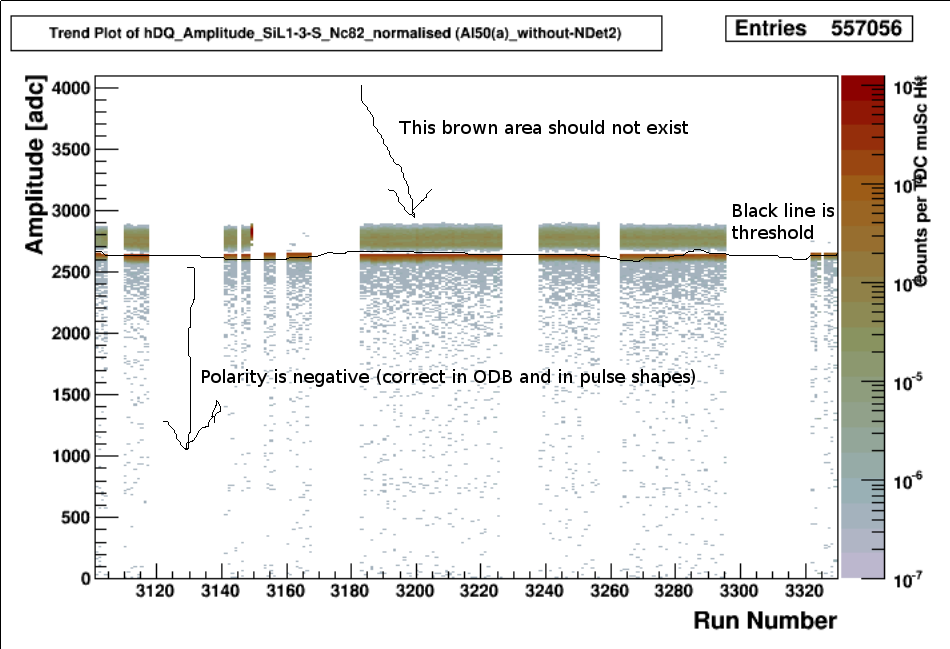
\includegraphics[width=0.9\linewidth]{figs/al50a/amplitude_too_low}
  \caption{The problem is best described in the figure. It has been dealt with in \issue{92}.}
  \label{fig:al50a_amp_below_thresh}
\end{figure}


\subsubsection{Pedestals Zero for Run 3257}
\label{sec:al50a_ped_zero}
The pedestals seem to drop to zero for run 3257, as can be seen in \ref{fig:al50a_ped}. It is unknown
why this happened. But the runs immediately after this (not included in the dataset) were strange themselves.

\begin{figure}
  \centering
  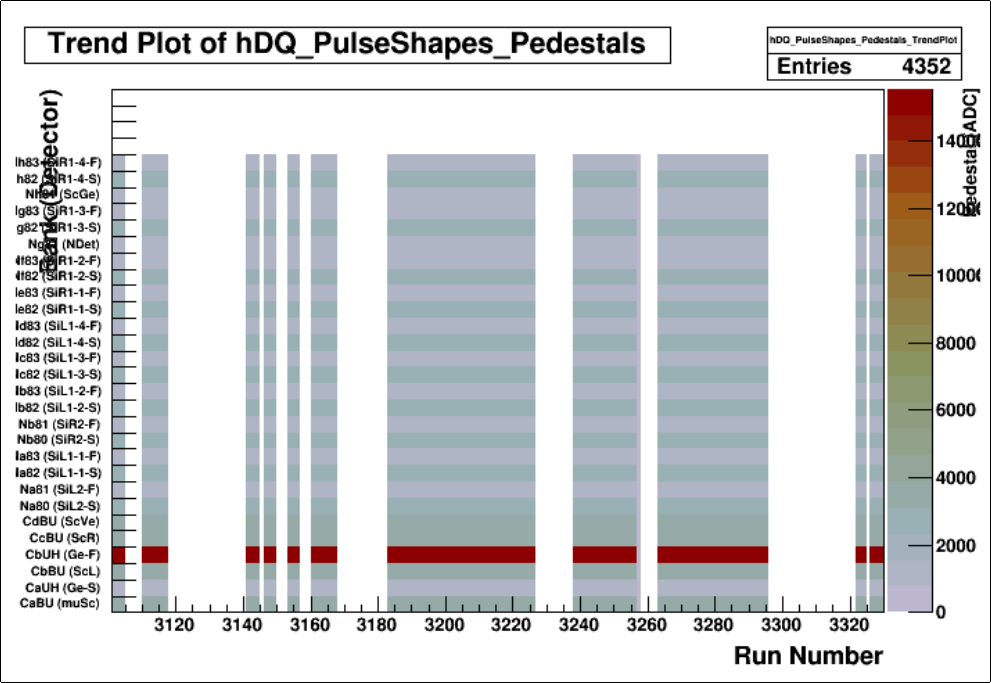
\includegraphics[width=0.9\linewidth]{figs/al50a/ped}
  \caption{Attention to the vertical band at 3257, where the pedestals drop inexplicably.}
  \label{fig:al50a_ped}
\end{figure}

\subsubsection{Crates Crash}
\label{sec:al50a_crate_crash}
Crate 5 and 6 crashed during run 3117, and a significant drop in rates can be seen.

\subsubsection{Inconsistent Rates 3183-3257}
\label{sec:al50a_rates}
In the figure \ref{fig:al50a_rates} we can see the fast silicon channels have rates that seem to vary quite a bit between runs 3183-3257.
This has not been explained, but the fast channels were notorious. The high rates caused some timestamp bunching and overflow, which
can be seen in \ref{fig:al50a_overflow}.

\begin{figure}
  \centering
  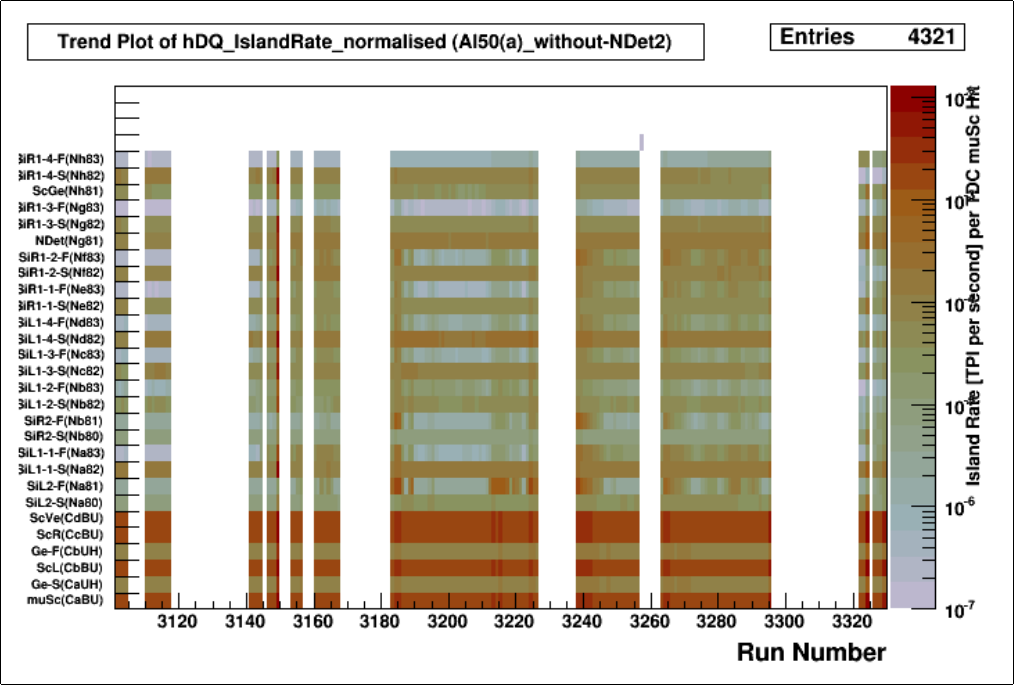
\includegraphics[width=0.9\linewidth]{figs/al50a/rates.png}
  \caption{The rates drop due to a crate crash in run 3117, the fast silicon rates are incocnsistent for runs 3183-3257.}
  \label{fig:al50a_rates}
\end{figure}

\begin{figure}
  \centering
  \begin{subfigure}{0.5\textwidth}
    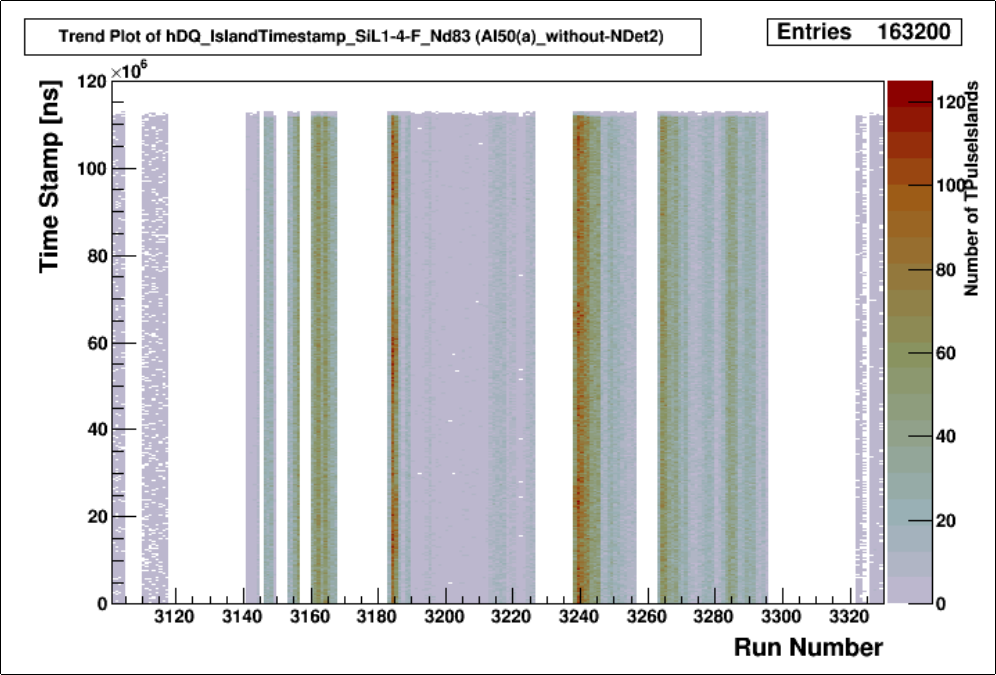
\includegraphics[width=0.9\linewidth]{figs/al50a/sil14f_timestamps}
  \end{subfigure}%
  \begin{subfigure}{0.5\textwidth}
    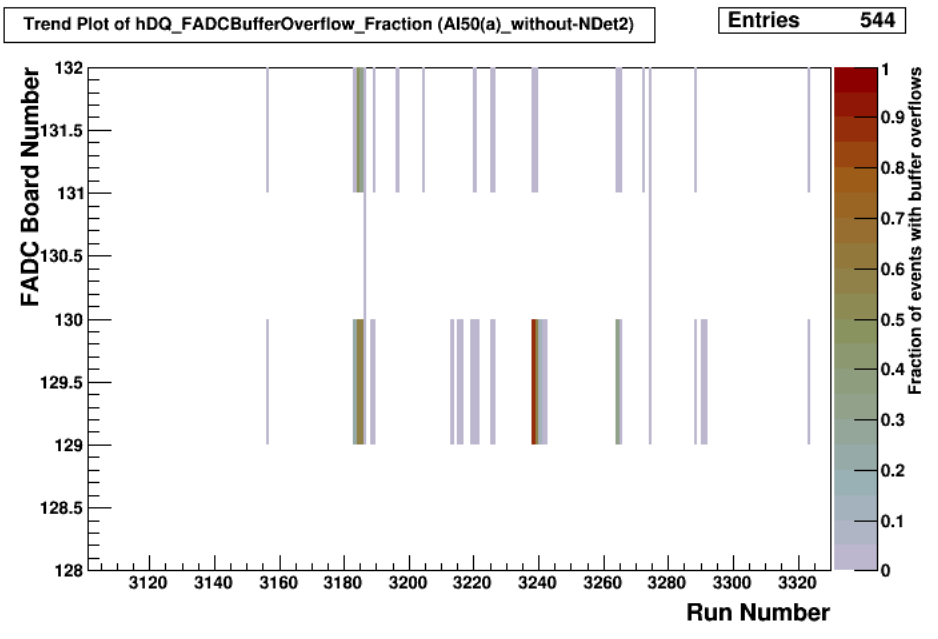
\includegraphics[width=0.9\linewidth]{figs/al50a/buffer_overflow}
  \end{subfigure}
  \caption{The buffer buffer's overflowing and signature timestamp bunching for a small fraction of the runs.}
  \label{fig:al50a_overflow}
\end{figure}


\subsubsection{Odd run 3150}
It looks as if a drop in the beam could have caused this, as the following run was specifically not included due
to the primary beam turning off. The data rate was abnormally low, and the duration as well. This latter point
could have occured because we stopped the run manually after noticing the low beam rate.


\subsection{Conclusions}
Either look into issue \ref{sec:al50a_tpi_length_incosnsistent} or cut out the runs that have the dip. Same thing with run 3257 of
problem \ref{sec:al50a_ped_zero}. Section \ref{sec:al50a_crate_crash} motivates us getting rid of run 3117 as well. Finally
the runs that had buffer overflows and timestamp bunching probably shouldn't be treated the same as the rest, so perhaps
we should also cut out those indicated in \ref{sec:al50a_rates}.

Keep all other runs, but look into the issues just in case.


%%%%%%%%%%%%%%%%%%%%%%%%%%%%%%%%%%%%%%%%%%%%%%%%%%%%%%%%%%%%%%%

\section{Al50 - B}
\begin{itemize}
  \item Aluminum
  \item 50 $\mu$ thick
  \item 10 cm $\times$ 10 cm
  \item Momentum scale factor 1.07
  \item Runs:
    3563-3646, 3650, 3667-3740
\end{itemize}

\subsection{Issues}
\subsubsection{S1R1-F and SiL1-F muScTDiff peak weak}

The peak in the muScTDiff plot is weaker for the first ~15 runs for the thick slow silicon channels. This
is odd because their slow channel rates are actually higher. See \ref{fig:al50b_rates}.

\begin{figure}
  \centering
  \begin{subfigure}{0.5\textwidth}
    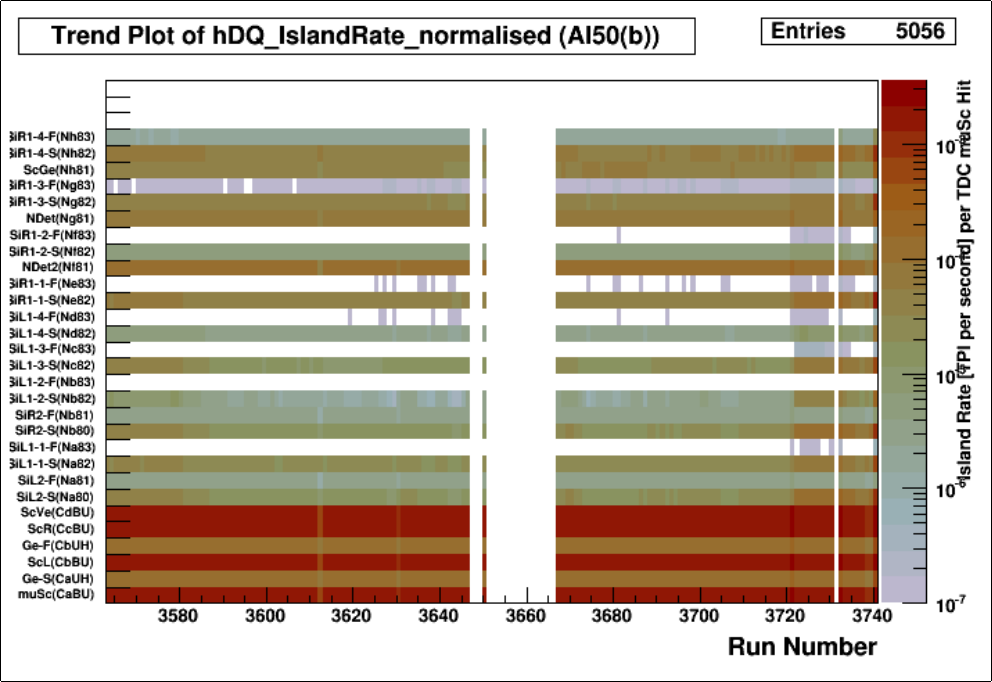
\includegraphics[width=0.9\linewidth]{figs/al50b/rates}
  \end{subfigure}%
  \begin{subfigure}{0.5\textwidth}
    \includegraphics[width=0.0\linewidth]{figs/al50b/sil2f_tdiff}
  \end{subfigure}
  \caption{The rates for SiR2-S and SiL2-S are higher according to the rate plot on the left;
    hoewver on the right we cannot see the peak in the timing correlation because of
    seemingly poor statistics.}
\end{figure}


\subsubsection{Peak in Amplitude Histograms}

There is a peak in the SiL1-f-S amplitude plot that appears in many datasets, but has
thusfar been uncharacterized. See \ref{fig:sil14s_amp}.

\begin{figure}
  \centering
  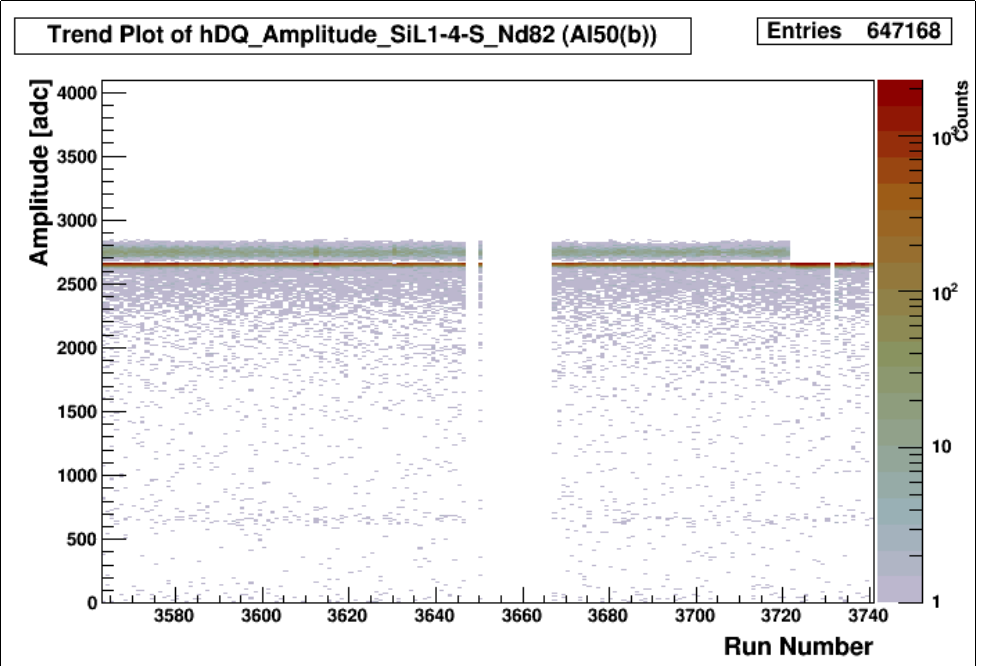
\includegraphics[width=0.9\linewidth]{figs/al50b/sil14s_amp}
  \caption{Around vertical 600 you can see what appears to be a band,
    suggesting for some reason pulses tend to have an amplitude of this.
    This has not been investigated yet.}
  \label{fig:sil14s_amp}
\end{figure}


\subsubsection{Run 3732}

This occured just after a crash of some crate, and has a livetime fraction
greater than 100\%.


\subsubsection{Noisy Thick Silicon Slow}

The noise really spikes up in later runs in SiL2-S and SiR2-S, which can be seen in \ref{fig:al50b_noise}.

\begin{figure}
  \centering
  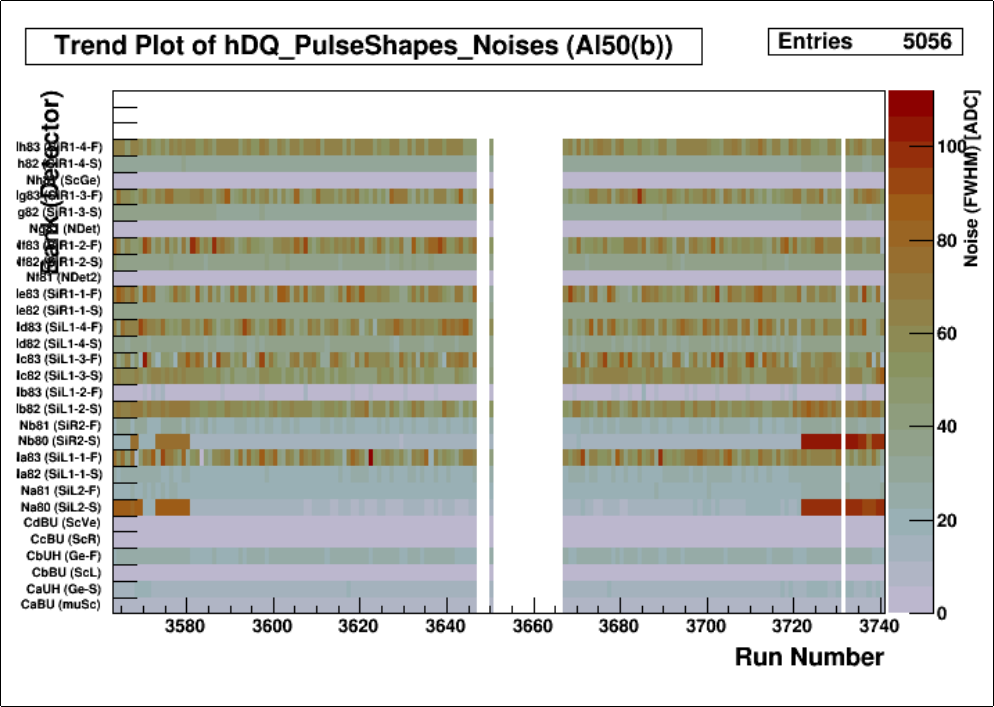
\includegraphics[width=0.9\textwidth]{figs/al50b/noise}
  \caption{The noise in the thick silicon detectors picks up near the end of this dataset.}
  \label{fig:al50b_noise}
\end{figure}


\subsubsection{Run 3612}

This run has strange rates. For one, the muSc rates are lower as seen in \ref{fig:al50b_rates}.
However, if we look at a timestamp distribution like in \ref{fig:al50b_gef_timestamps} to
see that the normalized rates are higher in many detectors. This run was ~3 times longer
than a normal run.


\subsection{Conclusion}

Toss out runs 3732 and 3612. Look into these issues.


%%%%%%%%%%%%%%%%%%%%%%%%%%%%%%%%%%%%%%%%%%%%%%%%%%%%%%%%%%%%%%%

\section{SiR Target}
\begin{itemize}
  \item Silicon
  \item 1500 $\mu$m thick
  \item 5 cm $\times$ 5 cm
  \item Momentum scale factor 1.30
  \item Runs:
    2091-2103, 2119-2172
\end{itemize}

%%%%%%%%%%%%%%%%%%%%%%%%%%%%%%%%%%%%%%%%%%%%%%%%%%%%%%%%%%%%%%%

\section{SiR2 - 1\%}
\begin{itemize}
  \item Silicon
  \item 1500 $\mu$m thick
  \item 5 cm $\times$ 5 cm
  \item Momentum scale factor 1.32
  \item Runs:
    3771, 3773-3779
\end{itemize}
%%%%%%%%%%%%%%%%%%%%%%%%%%%%%%%%%%%%%%%%%%%%%%%%%%%%%%%%%%%%%%%
\section{SiR2 - 3\%}
\begin{itemize}
  \item Silicon
  \item 1500 $\mu$m thick
  \item 5 cm $\times$ 5 cm
  \item Momentum scale factor 1.32
  \item Runs:
    3763-3770
\end{itemize}
%%%%%%%%%%%%%%%%%%%%%%%%%%%%%%%%%%%%%%%%%%%%%%%%%%%%%%%%%%%%%%%
\section{Si16P}
\begin{itemize}
  \item Silicon
  \item 65 $\mu$m thick
  \item 5 cm $\times$ 5 cm
  \item Momentum scale factor 1.06
  \item Runs:
    3474-3489, 3491-3540
\end{itemize}



\end{document}
